% ml_methods_companion.tex -- Cadence (ENGF0031 Scenario 2)
% Companion notes to the Accuracy Worksheet: how ML/AI is used in the ankle
% freeze-of-gait detector, the metrics we report, and how we interpret the model.
% Build:  tectonic ml_methods_companion.tex   (run from the worksheet/ folder)
% Every number is REAL -- computed from the Daphnet benchmark via leave-one-
% subject-out (LOSO); figures are produced by the scripts named in the footer.
\documentclass[11pt]{article}

\usepackage[a4paper,margin=2cm]{geometry}
\usepackage{amsmath,amssymb}
\usepackage{graphicx}
\usepackage{booktabs}
\usepackage{longtable}
\usepackage{array}
\usepackage{xcolor}
\usepackage{tikz}
\usepackage{caption}
\usepackage{enumitem}
\usepackage{microtype}
\usepackage{parskip}
\usetikzlibrary{positioning,arrows.meta,calc,shapes.geometric,backgrounds,fit}

\graphicspath{{../pi/accuracy_figs/}}

% ---- palette (matches the matplotlib figures) ------------------------------
\definecolor{navy}{HTML}{1F3A63}     % models / primary
\definecolor{freeze}{HTML}{B2182B}   % decision / cue
\definecolor{cSense}{HTML}{1C7293}   % sensing  (teal)
\definecolor{cEval}{HTML}{8A6D00}    % evaluation (amber)
\definecolor{cInterp}{HTML}{5B3A8C}  % interpretability (purple)
\definecolor{mute}{HTML}{56606B}

\captionsetup{font=small,labelfont=bf,labelsep=period}
\setlist{nosep,leftmargin=1.3em}

\newcommand{\feat}[1]{\texttt{\small #1}}
\newcommand{\code}[1]{\texttt{\small #1}}

% one CNN tensor "volume" centred at (#1,0): #2 half-width, #3 half-height,
% #4 front style, #5 back style.  An offset back face + front face reads as a
% 3-D slab; block height is used to suggest the channel count.
\newcommand{\cnnvol}[5]{%
  \filldraw[#5] ({#1-#2+0.15},{-#3+0.15}) rectangle ({#1+#2+0.15},{#3+0.15});%
  \filldraw[#4] ({#1-#2},{-#3}) rectangle ({#1+#2},{#3});%
}

% ===========================================================================
\begin{document}

\begin{center}
  {\LARGE\bfseries\color{navy} Cadence: Machine-Learning Methods \& Interpretability}\\[4pt]
  {\large How AI powers the ankle freeze-of-gait garment}\\[6pt]
  {\color{mute}\small Companion notes to the Accuracy Worksheet \,\textbar\; ENGF0031 Scenario 2 (Smart Clothing)}
\end{center}

\vspace{2pt}
\noindent\textbf{Purpose.} This companion explains \emph{how} machine learning and AI are used in
the Cadence detector, defines the accuracy metrics we report and why, and shows
how we interpret what the model has learned. Cadence senses gait from a single
ankle accelerometer and fires a vibrotactile cue when it detects a
\emph{freeze of gait} (FoG). Every figure and number here is computed from the
public \textbf{Daphnet} FoG benchmark using \textbf{leave-one-subject-out}
evaluation --- a model is never tested on a patient it trained on --- so the
numbers estimate performance on a \emph{new} wearer. Nothing is fabricated; the
scripts that generate each figure are listed on the last page.

% ===========================================================================
\section{How machine learning \& AI are applied in this project}

\subsection{The clinical problem, and why we use ML}
Freeze of gait is a sudden, involuntary inability to step --- the feeling that
the feet are ``glued to the floor.'' It is a leading cause of falls in
Parkinson's disease. A well-timed rhythmic \emph{cue} (here, a buzz on the
ankle) can help the wearer break the freeze and step off. The engineering task
is therefore: \emph{detect a freeze within a second or two, from one on-body
accelerometer, in real time.}

The classic hand-built rule is the \emph{Freeze Index} --- the ratio of power in
a ``freeze'' band ($3$--$8$\,Hz) to a ``locomotion'' band ($0.5$--$3$\,Hz). It
works on average, but the threshold that suits one patient's gait misfires on
another's. This is exactly where \textbf{supervised machine learning} helps: we
show the model many labelled windows of real accelerometer data and let it
\emph{learn} the freeze pattern --- including patient-to-patient variation ---
rather than hard-coding one rule. That learned pattern is the AI behind Cadence.

\begin{figure}[h]
  \centering
  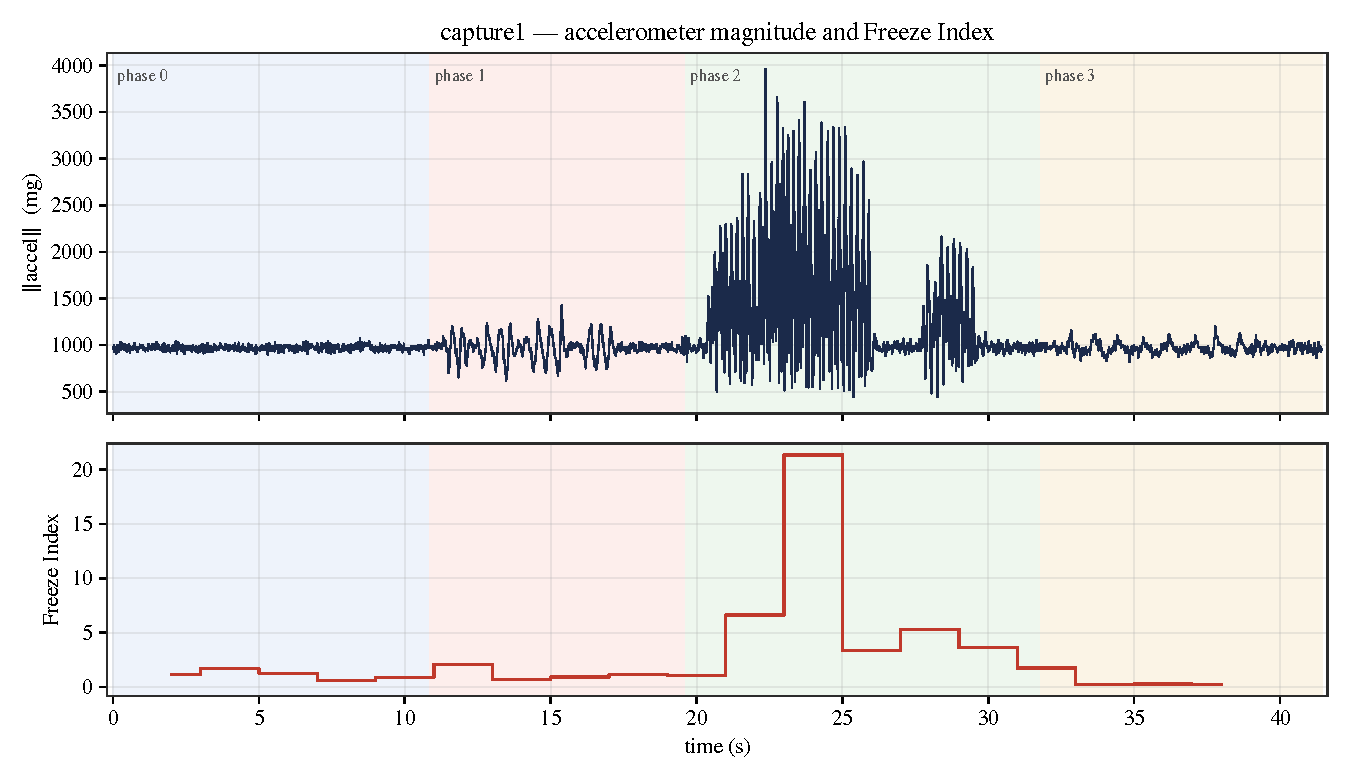
\includegraphics[width=0.82\textwidth]{capture1_trace}
  \caption{The raw signal the detector sees, from our own $\sim$41\,s ankle
  capture (phases shaded: still, walk, freeze, walk). \emph{Top:} accelerometer
  magnitude; \emph{bottom:} the textbook Freeze Index. During the freeze the
  signal becomes a high-frequency tremor-in-place and the Freeze Index spikes
  --- but note the index is noisy, which is why a learned model does better.}
  \label{fig:trace}
\end{figure}

\subsection{Two models, two different jobs}
We deliberately use \emph{two} models, because ``accurate'' and ``explainable''
pull in different directions:

\begin{itemize}
  \item \textbf{FoGNet --- a 1-D convolutional neural network ($\sim$18k
  parameters)} reads the raw $3\times256$ accelerometer window (4\,s at 64\,Hz)
  and learns its own filters end-to-end. \emph{This is the deployed detector},
  and its LOSO sensitivity/specificity are the headline result.
  \item \textbf{A 9-feature random forest (RF)} is trained on interpretable,
  hand-engineered features (band powers, jerk, magnitude statistics, dominant
  frequency, Freeze Index). It is \emph{not} deployed --- it is our
  ``\emph{glass box}'': because each input has a physical meaning, we can use
  SHAP, permutation importance and partial dependence (\S4) to see \emph{what in
  the signal} drives a ``freeze'' decision, and to sanity-check the CNN.
\end{itemize}

\subsection{The whole picture at a glance}
Figure~\ref{fig:mindmap} maps the five things ML/AI touches in this project:
sensing, the two models, the decision logic, honest evaluation, and
interpretability. Figure~\ref{fig:pipeline} then traces the live closed loop a
single window travels through.

\begin{figure}[h]
  \centering
  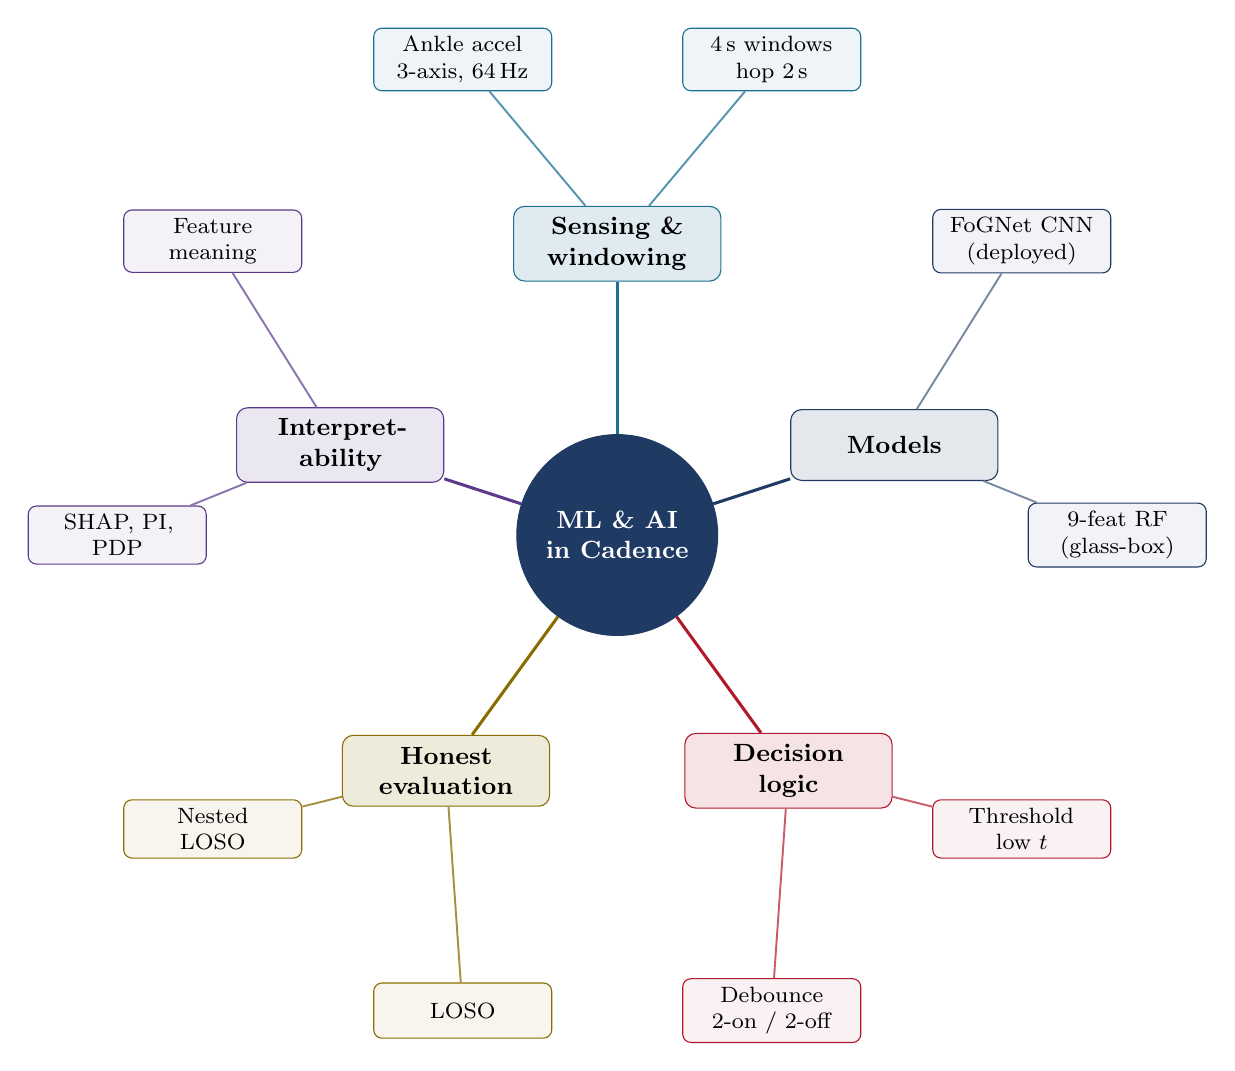
\begin{tikzpicture}[
    core/.style={circle, draw=navy, fill=navy, text=white,
                  font=\bfseries\small, align=center, minimum size=2.55cm,
                  inner sep=1pt},
    branch/.style 2 args={rounded corners=4pt, align=center,
                  font=\small\bfseries, text=black, text width=2.35cm,
                  minimum height=0.9cm, inner sep=4pt, draw=#1, fill=#2},
    leaf/.style 2 args={rounded corners=3pt, align=center, font=\footnotesize,
                  text=black, text width=2.05cm, minimum height=0.7cm,
                  inner sep=3pt, draw=#1, fill=#2},
    spoke/.style={line width=1.1pt, #1},
    twig/.style={line width=0.7pt, #1},
  ]
    \node[core] (c) at (0,0) {ML \& AI\\in Cadence};

    % --- five branches at 72 deg spacing -----------------------------------
    \node[branch={cSense}{cSense!14}]  (b1) at (90:3.7)  {Sensing \&\\windowing};
    \node[branch={navy}{navy!12}]      (b2) at (18:3.7)  {Models};
    \node[branch={freeze}{freeze!12}]  (b3) at (-54:3.7) {Decision\\logic};
    \node[branch={cEval}{cEval!14}]    (b4) at (-126:3.7){Honest\\evaluation};
    \node[branch={cInterp}{cInterp!12}](b5) at (162:3.7) {Interpret-\\ability};

    % --- ten leaves, evenly spaced every 36 deg, flanking their branch ------
    \node[leaf={cSense}{cSense!7}]   (l1a) at (108:6.35) {Ankle accel\\3-axis, 64\,Hz};
    \node[leaf={cSense}{cSense!7}]   (l1b) at (72:6.35)  {4\,s windows\\hop 2\,s};
    \node[leaf={navy}{navy!6}]       (l2a) at (36:6.35)  {FoGNet CNN\\(deployed)};
    \node[leaf={navy}{navy!6}]       (l2b) at (0:6.35)   {9-feat RF\\(glass-box)};
    \node[leaf={freeze}{freeze!6}]   (l3a) at (-36:6.35) {Threshold\\low $t$};
    \node[leaf={freeze}{freeze!6}]   (l3b) at (-72:6.35) {Debounce\\2-on / 2-off};
    \node[leaf={cEval}{cEval!7}]     (l4a) at (-108:6.35){LOSO};
    \node[leaf={cEval}{cEval!7}]     (l4b) at (-144:6.35){Nested\\LOSO};
    \node[leaf={cInterp}{cInterp!7}] (l5a) at (180:6.35) {SHAP, PI,\\PDP};
    \node[leaf={cInterp}{cInterp!7}] (l5b) at (144:6.35) {Feature\\meaning};

    % --- spokes (core->branch) and twigs (branch->leaf) --------------------
    \draw[spoke={cSense}]  (c)--(b1);  \draw[spoke={navy}] (c)--(b2);
    \draw[spoke={freeze}]  (c)--(b3);  \draw[spoke={cEval}](c)--(b4);
    \draw[spoke={cInterp}] (c)--(b5);
    \draw[twig={cSense!75}]  (b1)--(l1a); \draw[twig={cSense!75}]  (b1)--(l1b);
    \draw[twig={navy!60}]    (b2)--(l2a); \draw[twig={navy!60}]    (b2)--(l2b);
    \draw[twig={freeze!70}]  (b3)--(l3a); \draw[twig={freeze!70}]  (b3)--(l3b);
    \draw[twig={cEval!75}]   (b4)--(l4a); \draw[twig={cEval!75}]   (b4)--(l4b);
    \draw[twig={cInterp!70}] (b5)--(l5a); \draw[twig={cInterp!70}] (b5)--(l5b);
  \end{tikzpicture}
  \caption{Mind map of where machine learning and AI enter the Cadence project.
  Each coloured branch is one theme; the outer nodes are the concrete pieces.
  Sensing feeds the two \emph{models}; the model's probability is turned into an
  action by the \emph{decision logic}; \emph{honest evaluation} keeps the
  reported numbers fair; \emph{interpretability} explains what was learned.}
  \label{fig:mindmap}
\end{figure}

\begin{figure}[h]
  \centering
  \resizebox{\textwidth}{!}{%
  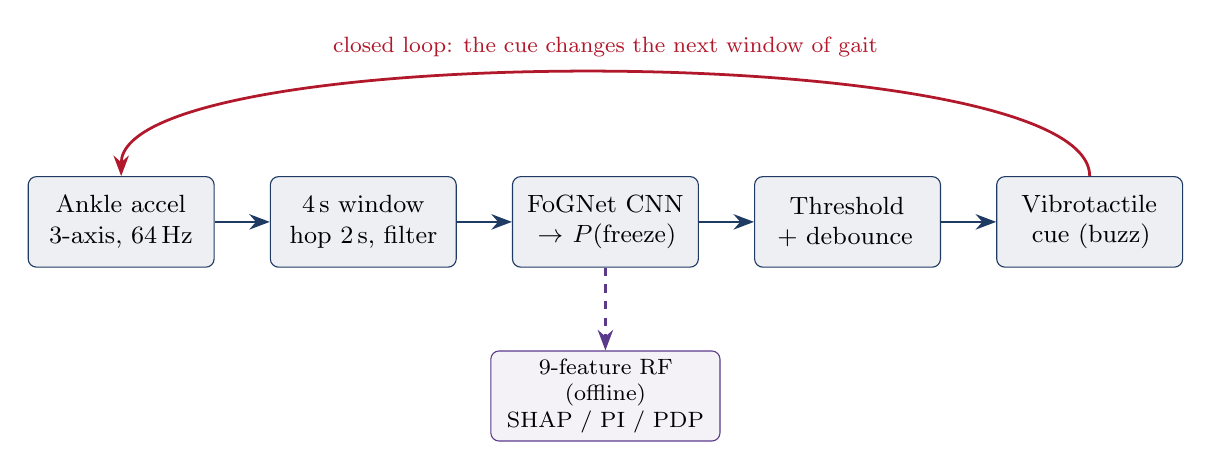
\begin{tikzpicture}[
    stage/.style={rounded corners=3pt, draw=navy, fill=navy!8, align=center,
                  font=\small, text width=2.15cm, minimum height=1.15cm,
                  inner sep=3pt},
    off/.style={rounded corners=3pt, draw=cInterp, fill=cInterp!7, align=center,
                font=\footnotesize, text width=2.7cm, minimum height=1.0cm,
                inner sep=3pt},
    fl/.style={-{Stealth[length=2.6mm]}, line width=1pt, navy},
  ]
    \node[stage] (s1) {Ankle accel\\3-axis, 64\,Hz};
    \node[stage, right=0.7cm of s1] (s2) {4\,s window\\hop 2\,s, filter};
    \node[stage, right=0.7cm of s2] (s3) {FoGNet CNN\\$\to P(\mathrm{freeze})$};
    \node[stage, right=0.7cm of s3] (s4) {Threshold\\$+$ debounce};
    \node[stage, right=0.7cm of s4] (s5) {Vibrotactile\\cue (buzz)};
    \draw[fl] (s1)--(s2); \draw[fl] (s2)--(s3);
    \draw[fl] (s3)--(s4); \draw[fl] (s4)--(s5);
    \node[off, below=1.05cm of s3] (rf)
       {9-feature RF\\(offline)\\SHAP / PI / PDP};
    \draw[fl, cInterp, dashed] (s3)--(rf);
    % closed-loop feedback arc routed OVER THE TOP, so it never crosses the RF
    % node that sits below the chain (avoids the earlier text-on-text overlap).
    \draw[fl, freeze]
       (s5.north) .. controls +(0,1.75) and +(0,1.75) .. (s1.north)
       node[midway, above=2pt, font=\footnotesize, text=freeze]
       {closed loop: the cue changes the next window of gait};
  \end{tikzpicture}}
  \caption{The live pipeline one window travels through. Raw ankle acceleration
  is buffered into a 4\,s window, the CNN outputs a freeze probability, a
  \emph{low} threshold plus debouncing (assert after 2 positive windows, release
  after 2 clear --- matching the firmware) decides whether to buzz. The buzz
  feeds back into the wearer's gait, closing the loop. The random forest sits
  \emph{off} the live path: it exists only to explain the signal.}
  \label{fig:pipeline}
\end{figure}

\clearpage
% ===========================================================================
\section{Categorising windows \& finding the best parameters}

\subsection{Categorising = drawing a boundary on a probability surface}
A classifier does not output ``freeze'' or ``not'' directly --- it outputs a
\emph{probability} $P(\mathrm{freeze})$ for each window. We ``categorise'' by
comparing that probability to a \emph{threshold} $t$: buzz if
$P(\mathrm{freeze})\ge t$. Figure~\ref{fig:contour} shows this surface over two
example features. The coloured shading is the probability; a contour line of
constant probability \emph{is} the decision boundary, and choosing $t$ simply
slides that line. Because freezes are rare (only $9.5\%$ of windows), the useful
boundary is the \emph{low} green contour ($t\!\approx\!0.1$), not the textbook
$0.5$: at $0.5$ we would only flag the small, very-high-jerk pocket and miss most
freezes.

\begin{figure}[h]
  \centering
  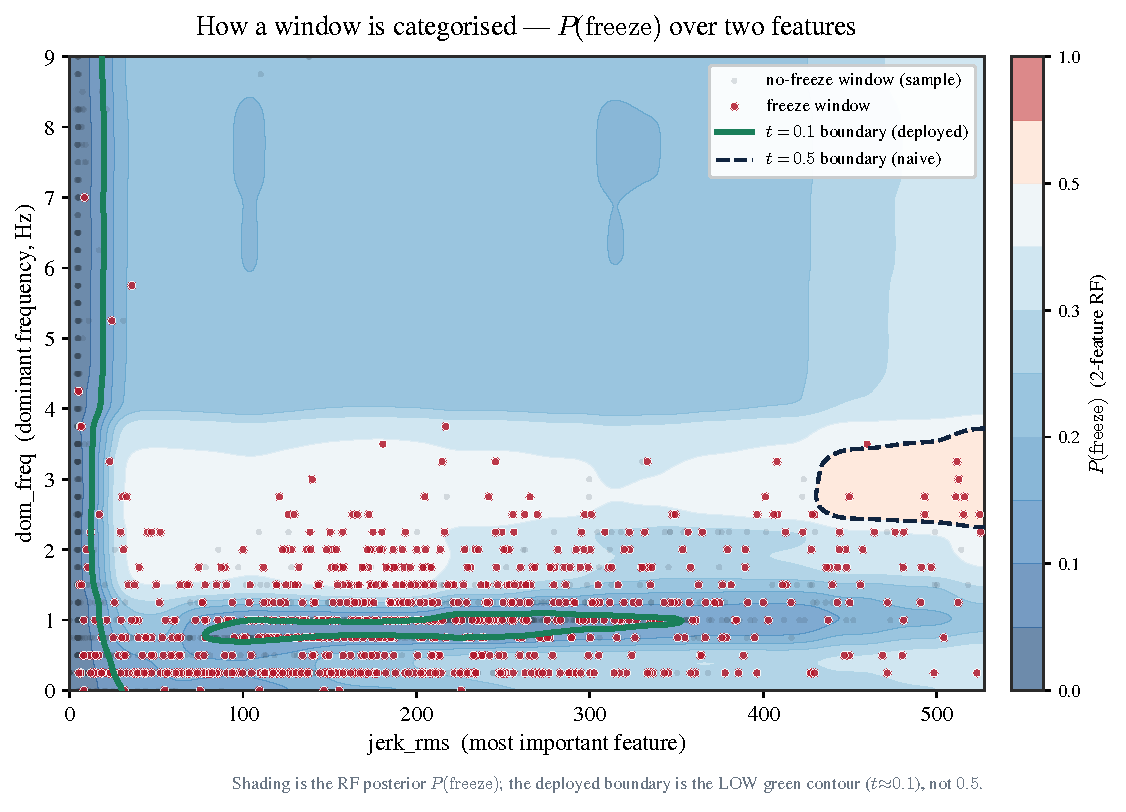
\includegraphics[width=0.78\textwidth]{decision_contour}
  \caption{\textbf{How a window is categorised.} The random forest's posterior
  $P(\mathrm{freeze})$ over two real features (\feat{jerk\_rms} and
  \feat{dom\_freq}), with every real window overlaid (freezes in red, a sample of
  non-freezes as a haze). Freezes concentrate at high jerk and low dominant
  frequency. Lowering the threshold from the dashed $0.5$ line to the solid green
  $t\!\approx\!0.1$ line enlarges the ``freeze'' region --- trading specificity
  for the sensitivity we need.}
  \label{fig:contour}
\end{figure}

\subsection{Finding the best parameters --- there are two kinds}
``Best parameters'' means two different things, and we tune them separately.

\paragraph{(a) Model complexity (hyper-parameters).}
How deep should each tree be? How many samples per leaf? Too simple and the model
underfits; too complex and it memorises the training subjects and fails on a new
one. We grid-search these with \emph{subject-grouped} 5-fold cross-validation
(Figure~\ref{fig:grid}) and keep the held-out optimum (here \feat{max\_depth}\,$=8$,
\feat{min\_samples\_leaf}\,$=16$). Grouping the folds by subject is the honest
part: the validation patients are never in the training folds.

\paragraph{(b) The decision threshold.}
Given a trained model, where do we put $t$? Sweeping it (Figure~\ref{fig:opp})
trades sensitivity against specificity. We pick the point that maximises
\emph{Youden's J} ($=\text{sensitivity}+\text{specificity}-1$); for the
interpretable RF this is $t^*\!\approx\!0.10$ (sensitivity $0.75$, specificity
$0.76$). The threshold-free ranking quality is summarised by ROC-AUC $=0.82$ and
PR-AUC $=0.33$.

\begin{figure}[h]
  \centering
  \begin{minipage}[t]{0.49\textwidth}
    \centering
    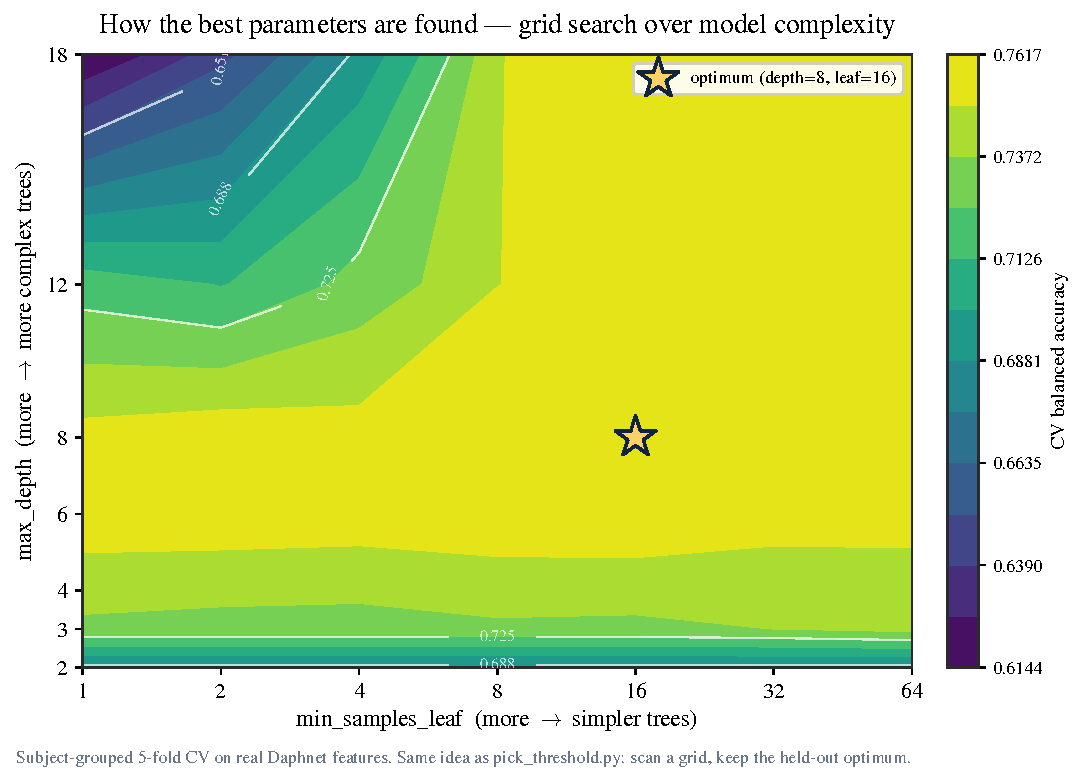
\includegraphics[width=\linewidth]{param_grid}
    \captionof{figure}{Hyper-parameter search. Subject-grouped CV balanced
    accuracy over tree depth $\times$ leaf size; the star is the held-out
    optimum. Both over- and under-complex corners score worse.}
    \label{fig:grid}
  \end{minipage}\hfill
  \begin{minipage}[t]{0.49\textwidth}
    \centering
    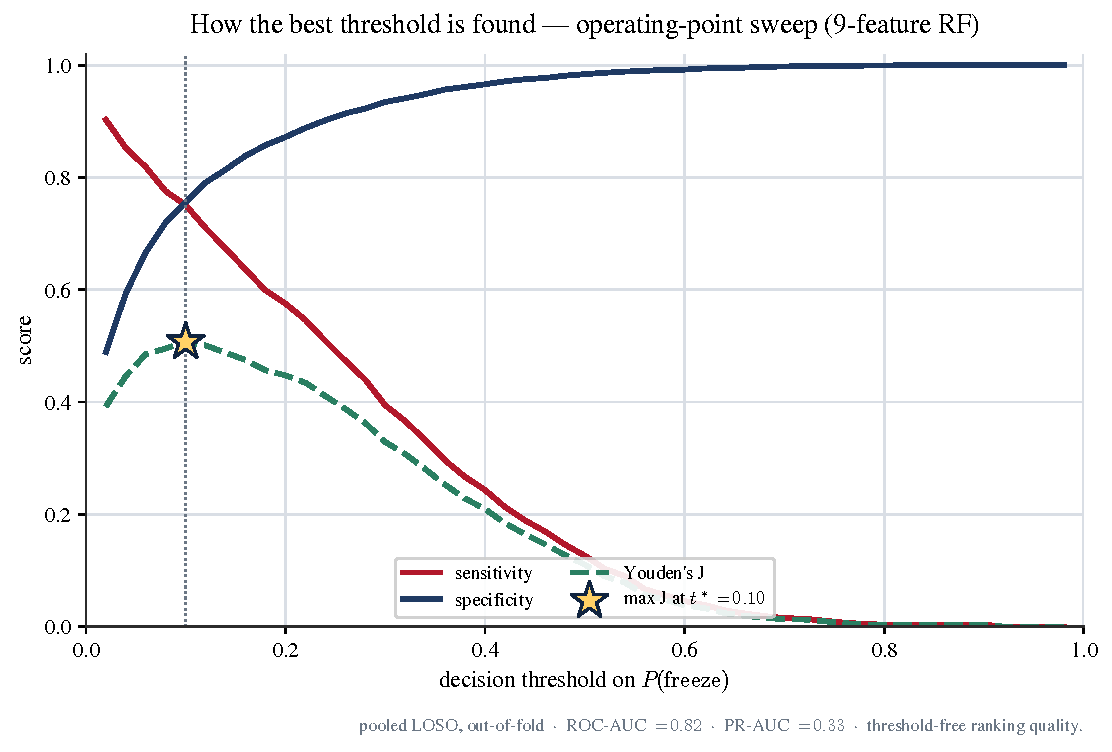
\includegraphics[width=\linewidth]{operating_point}
    \captionof{figure}{Threshold search. As $t$ rises, sensitivity falls and
    specificity rises; Youden's J peaks at $t^*\!\approx\!0.10$. This is exactly
    what \code{pick\_threshold.py} automates per subject.}
    \label{fig:opp}
  \end{minipage}
\end{figure}

\subsection{Why honest selection matters}
Both the threshold \emph{and} the hyper-parameters must be chosen on data that is
\textbf{disjoint by subject} from the data we score them on. If we scanned every
threshold on the whole pooled set and then quoted the best number from that
\emph{same} set, we would be tuning on the test data and over-reporting. Our
\code{pick\_threshold.py} does \emph{nested} LOSO --- it chooses $t$ on the other
patients, then scores the held-out one --- so the reported sensitivity and
specificity are what a genuinely \emph{new} patient should expect.

\clearpage
% ===========================================================================
\section{The 15 most useful accuracy metrics}

\subsection{Why ``accuracy'' is the wrong headline}
Freeze windows are rare ($9.5\%$). A lazy model that always says ``no freeze''
is therefore $\sim$$90\%$ \emph{accurate} while catching \emph{zero} freezes ---
useless for a cueing garment (Figure~\ref{fig:caveat}). Accuracy hides exactly
the failure we care about, so we headline \textbf{sensitivity} (freezes caught)
and \textbf{specificity} (calm gait correctly left alone) instead.

\begin{figure}[h]
  \centering
  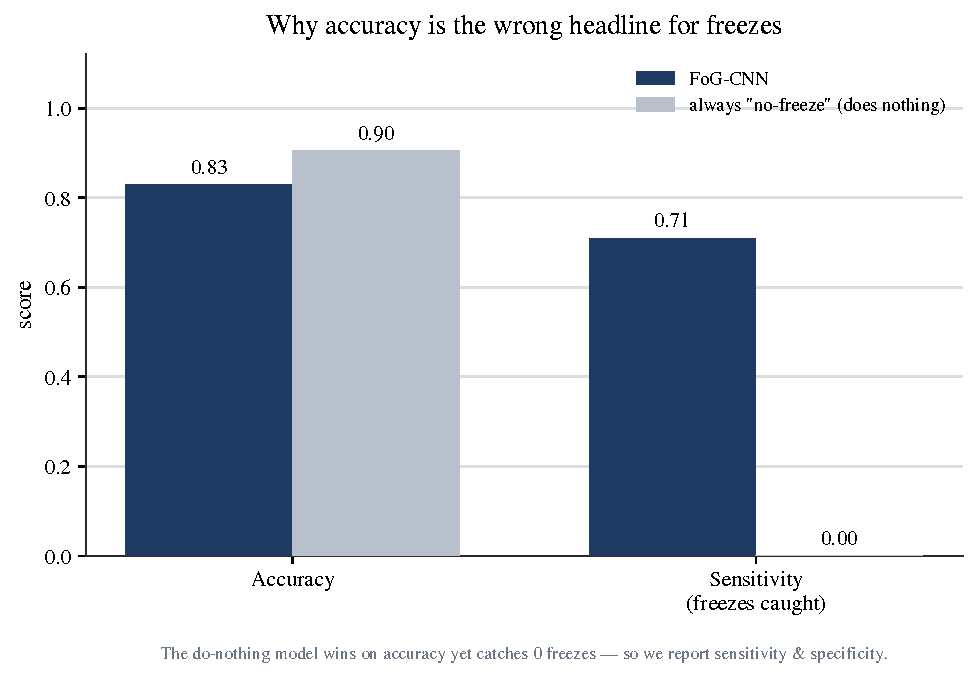
\includegraphics[width=0.66\textwidth]{accuracy_caveat}
  \caption{The accuracy trap. A do-nothing model ``wins'' on accuracy
  ($0.90$ vs $0.83$) yet has $0.00$ sensitivity --- it never cues a single
  freeze. This is why our headline metric is sensitivity \& specificity, not
  accuracy.}
  \label{fig:caveat}
\end{figure}

\subsection{The confusion matrix --- where every metric comes from}
All of the metrics below are arithmetic on four counts, with \emph{freeze} as the
positive class. From the deployed CNN's pooled LOSO predictions:
$\mathrm{TP}=607$ (freezes caught), $\mathrm{FP}=1285$ (false buzzes),
$\mathrm{FN}=248$ (missed freezes), $\mathrm{TN}=6842$ (calm correctly ignored),
over $N=8982$ windows.

\begin{figure}[h]
  \centering
  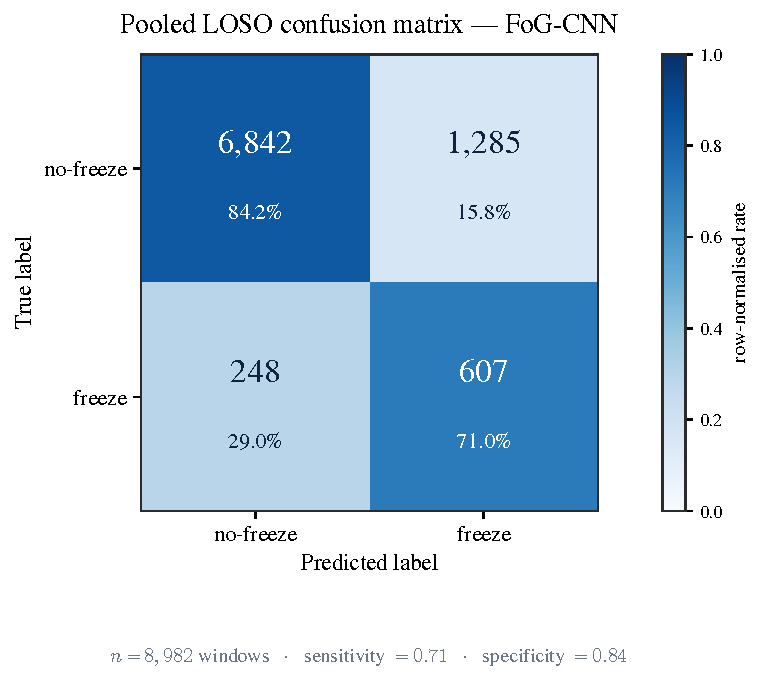
\includegraphics[width=0.50\textwidth]{confusion_matrix}
  \caption{Confusion matrix for the deployed FoG-CNN (pooled LOSO). Rows are the
  truth, columns the prediction; the off-diagonal cells are the two error types
  every metric trades against.}
  \label{fig:cm}
\end{figure}

\subsection{The fifteen metrics}
\textbf{Notation:} $\mathrm{TPR}$ = sensitivity, $\mathrm{TNR}$ = specificity,
$\mathrm{PPV}$ = precision; positive class = freeze. For MCC, let
$N_P=\mathrm{TP}{+}\mathrm{FN}$ (actual freezes), $N_N=\mathrm{TN}{+}\mathrm{FP}$,
$N_{\hat P}=\mathrm{TP}{+}\mathrm{FP}$ (predicted freezes),
$N_{\hat N}=\mathrm{TN}{+}\mathrm{FN}$. For $\kappa$, $p_o$ is observed agreement
(= accuracy) and $p_e$ is agreement expected by chance.

{\footnotesize
\setlength{\tabcolsep}{4pt}
\renewcommand{\arraystretch}{1.35}
\begin{longtable}{@{}p{2.45cm} p{3.05cm} >{\centering\arraybackslash}p{0.9cm} p{8.1cm}@{}}
\toprule
\textbf{Metric} & \textbf{Formula} & \textbf{Value} & \textbf{What it tells you (and why it matters here)}\\
\midrule
\endfirsthead
\toprule
\textbf{Metric} & \textbf{Formula} & \textbf{Value} & \textbf{What it tells you}\\
\midrule
\endhead
\midrule \multicolumn{4}{r}{\footnotesize\itshape continued on next page}\\
\endfoot
\bottomrule
\endlastfoot

\textbf{1. Sensitivity} \newline (recall, TPR) &
$\dfrac{\mathrm{TP}}{\mathrm{TP}+\mathrm{FN}}$ & \textbf{0.710} &
Fraction of real freezes the garment catches. \textbf{Headline \#1} --- a missed
freeze means no cue when the patient needs it.\\

\textbf{2. Specificity} \newline (TNR) &
$\dfrac{\mathrm{TN}}{\mathrm{TN}+\mathrm{FP}}$ & \textbf{0.842} &
Fraction of calm/normal gait correctly left alone. \textbf{Headline \#2} --- low
specificity means nuisance buzzes that annoy and get the device switched off.\\

3. Precision \newline (PPV) &
$\dfrac{\mathrm{TP}}{\mathrm{TP}+\mathrm{FP}}$ & 0.321 &
Of all the times we buzz, the fraction that were truly freezes. Looks low, but
that is the rare-class arithmetic (see prevalence): worth less here than recall.\\

4. NPV &
$\dfrac{\mathrm{TN}}{\mathrm{TN}+\mathrm{FN}}$ & 0.965 &
When the device stays silent, the chance the wearer really was not freezing ---
reassuringly high.\\

5. F1 score &
$\dfrac{2\,\mathrm{PPV}\cdot\mathrm{TPR}}{\mathrm{PPV}+\mathrm{TPR}}$ & 0.442 &
Harmonic mean of precision and recall --- one number when you must balance the
two, but it ignores the (large) true-negative count.\\

6. F2 score &
$\dfrac{5\,\mathrm{PPV}\cdot\mathrm{TPR}}{4\,\mathrm{PPV}+\mathrm{TPR}}$ & 0.571 &
Like F1 but weights \emph{recall} four times more than precision --- the right
emphasis for a safety cue where misses cost more than false alarms.\\

7. Balanced \newline accuracy &
$\tfrac{1}{2}(\mathrm{TPR}+\mathrm{TNR})$ & 0.776 &
Plain accuracy re-weighted as if the two classes were equal in size --- the
honest ``accuracy'' for imbalanced data.\\

8. MCC &
$\dfrac{\mathrm{TP\cdot TN}-\mathrm{FP\cdot FN}}{\sqrt{N_P\,N_N\,N_{\hat P}\,N_{\hat N}}}$
& 0.397 &
Correlation between prediction and truth using all four cells; $+1$ perfect, $0$
chance, $-1$ inverted. The most robust single score under class imbalance.\\

9. Cohen's $\kappa$ &
$\dfrac{p_o-p_e}{1-p_e}$ & 0.358 &
Agreement \emph{above chance}. Guards against being impressed by accuracy that a
coin-flip with the same base rate would also reach.\\

10. Youden's J &
$\mathrm{TPR}+\mathrm{TNR}-1$ & 0.552 &
Sensitivity $+$ specificity $-1$. A single ``how good is this operating point''
score; maximising it is how we pick the threshold (\S2).\\

11. LR$+$ &
$\dfrac{\mathrm{TPR}}{1-\mathrm{TNR}}$ & 4.49 &
A buzz multiplies the odds that the wearer is truly freezing by $\sim$$4.5\times$
--- the diagnostic ``weight'' of a positive.\\

12. LR$-$ &
$\dfrac{1-\mathrm{TPR}}{\mathrm{TNR}}$ & 0.345 &
Silence multiplies the odds of freezing by $\sim$$0.34$ --- i.e.\ makes a freeze
about $3\times$ less likely.\\

13. Miss rate \newline (FNR) &
$\dfrac{\mathrm{FN}}{\mathrm{TP}+\mathrm{FN}}$ & 0.290 &
Fraction of freezes we miss ($=1-$ sensitivity). The error we most want to drive
down for a fall-prevention device.\\

14. Fall-out \newline (FPR) &
$\dfrac{\mathrm{FP}}{\mathrm{FP}+\mathrm{TN}}$ & 0.158 &
Fraction of calm gait wrongly buzzed ($=1-$ specificity) --- the comfort/battery
cost of the device.\\

15. Prevalence &
$\dfrac{\mathrm{TP}+\mathrm{FN}}{N}$ & 0.095 &
Base rate of freeze windows. Explains why precision is modest and why accuracy is
the wrong headline.\\

\end{longtable}}

\begin{figure}[h]
  \centering
  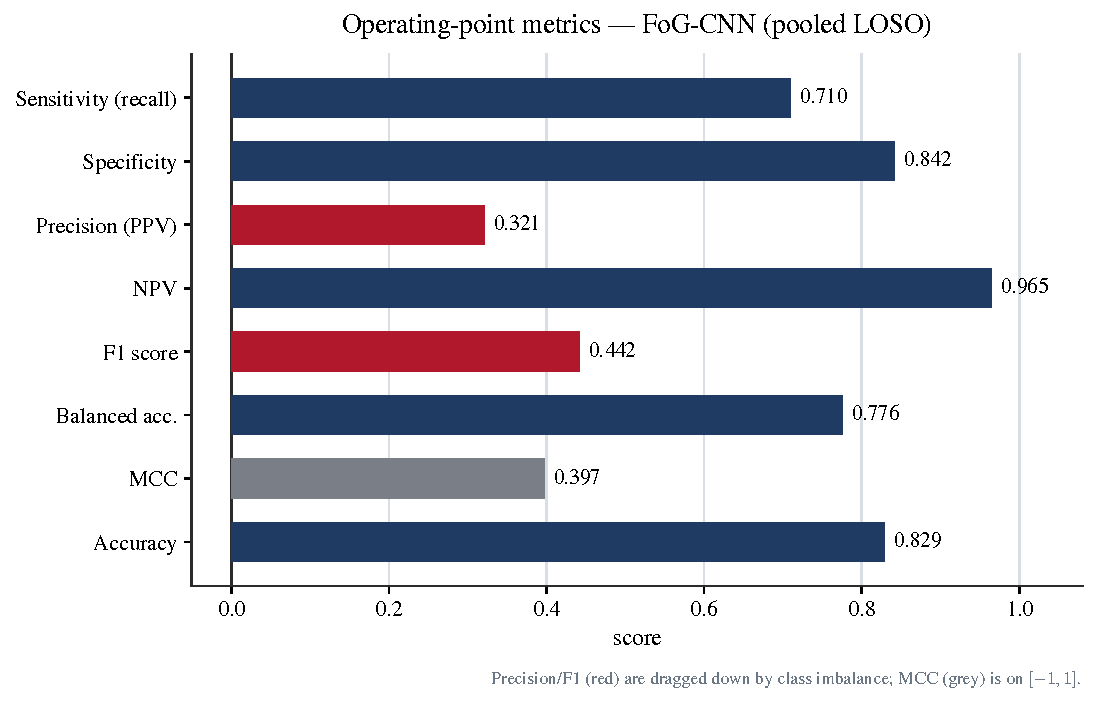
\includegraphics[width=0.84\textwidth]{metrics_panel}
  \caption{Eight of the key metrics at the deployed operating point. Sensitivity
  and specificity (navy, headline) sit well above chance; precision and F1 (red)
  are pulled down by the $9.5\%$ prevalence, not by a weak detector; MCC (grey)
  lives on $[-1,1]$.}
  \label{fig:panel}
\end{figure}

\noindent\textbf{Bottom line.} The deployed FoG-CNN reaches
\textbf{sensitivity $0.71$ / specificity $0.84$} on unseen patients (LOSO). We
accept modest precision because, for a safety cue, catching freezes (recall)
matters more than the occasional extra buzz.

\bigskip
% ===========================================================================
\section{Interpreting the model: SHAP, permutation importance, partial dependence}

These three tools answer \emph{different} questions about the glass-box random
forest, so they need not agree --- and where they differ is itself informative.

\begin{itemize}
  \item \textbf{Permutation importance (PI)} --- ``how much does held-out
  performance \emph{drop} if I randomly shuffle this one feature?'' A global,
  model-level, performance-based ranking.
  \item \textbf{SHAP} --- ``for \emph{this} window, how much did each feature push
  the prediction up or down?'' A local, additive attribution; averaging its
  magnitude gives a global view.
  \item \textbf{Partial dependence (PDP)} --- ``as I sweep one feature across its
  range, how does the average predicted $P(\mathrm{freeze})$ move?'' Shows the
  \emph{shape} and \emph{direction} of an effect.
\end{itemize}

\subsection{Global importance: what the model leans on}
Both rankings (Figures~\ref{fig:pi} and~\ref{fig:shapbar}) put \feat{jerk\_rms} --- the rate of change
of acceleration --- at or near the top, and SHAP makes it dominant (about twice
the next feature). Physically this fits: a freeze is a trembling, shuffling
``attempt to move'' at the ankle, which is rich in jerk. Note a subtlety:
\feat{total\_power} and \feat{freeze\_power} rank \emph{high} in permutation
importance but are \emph{flat} in PDP below --- they matter through
\emph{interactions} with other features, not through a simple one-feature trend.

\begin{figure}[h]
  \centering
  \begin{minipage}[t]{0.49\textwidth}
    \centering
    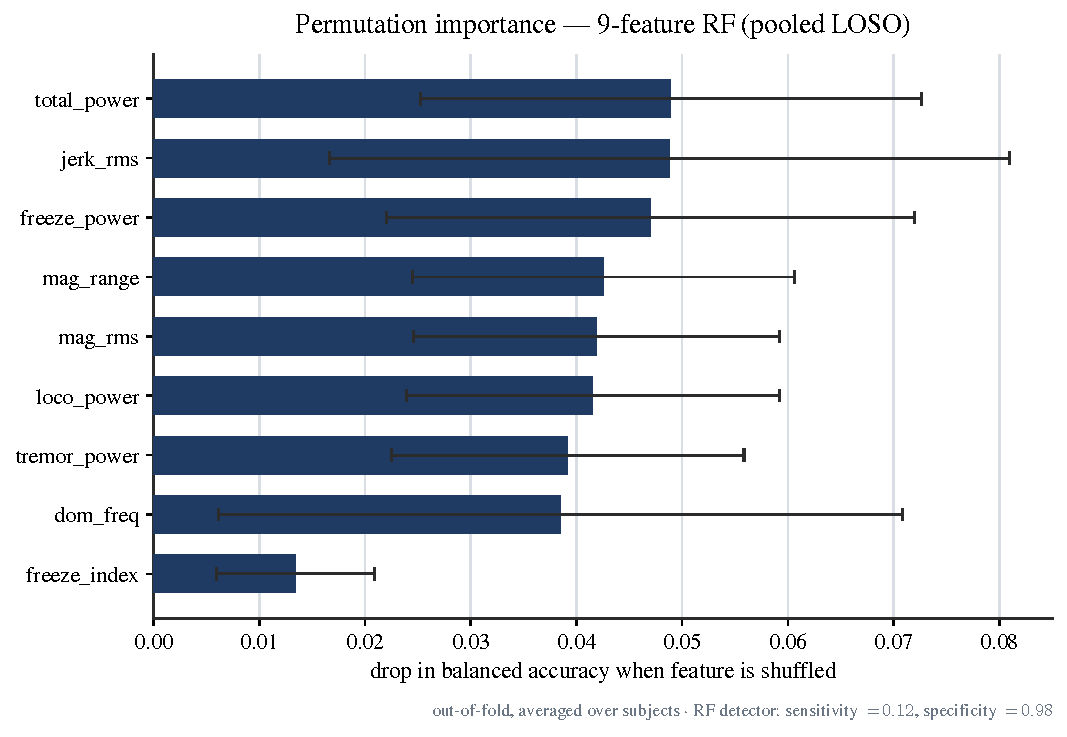
\includegraphics[width=\linewidth]{perm_importance}
    \captionof{figure}{Permutation importance: drop in balanced accuracy when
    each feature is shuffled. Top features overlap within their error bars; the
    Freeze Index ranks \emph{last}.}
    \label{fig:pi}
  \end{minipage}\hfill
  \begin{minipage}[t]{0.49\textwidth}
    \centering
    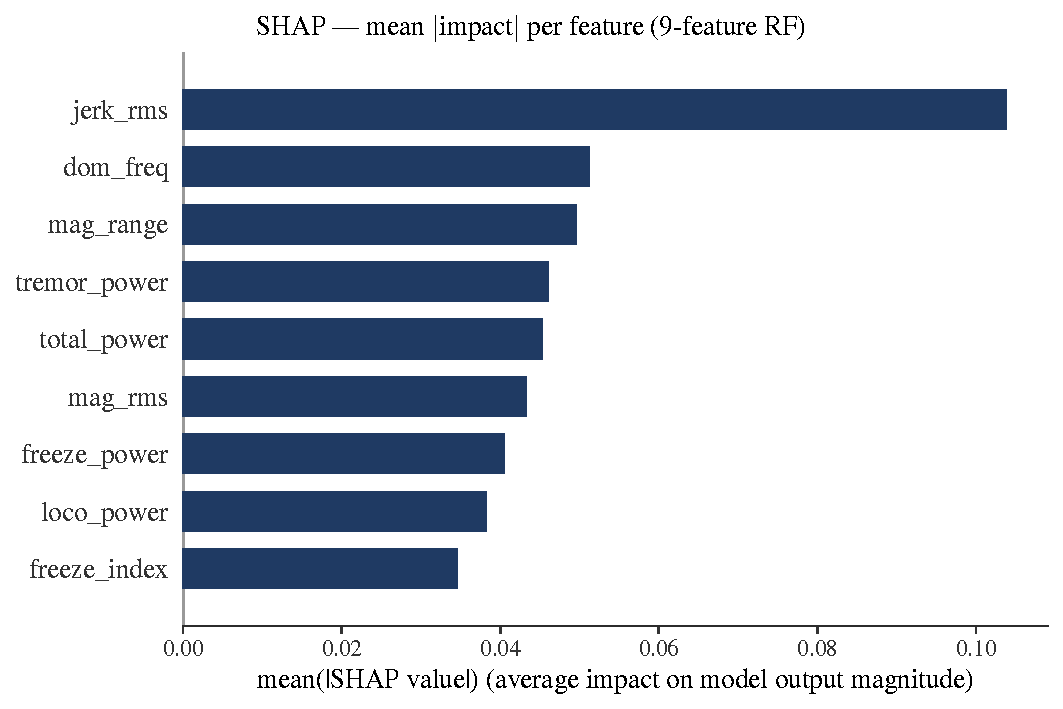
\includegraphics[width=\linewidth]{shap_bar}
    \captionof{figure}{Mean $|$SHAP$|$ per feature. \feat{jerk\_rms} dominates
    ($\sim$2$\times$ the next); the Freeze Index is again last.}
    \label{fig:shapbar}
  \end{minipage}
\end{figure}

\subsection{Direction \& spread: which way each feature pushes}
The SHAP beeswarm (Figure~\ref{fig:bee}) colours each window by its feature value.
For \feat{jerk\_rms}, high values (red) sit on the positive side --- they push the
prediction \emph{towards} freeze --- and its spread is the widest, confirming it is
the strongest, most consistent driver.

\begin{figure}[h]
  \centering
  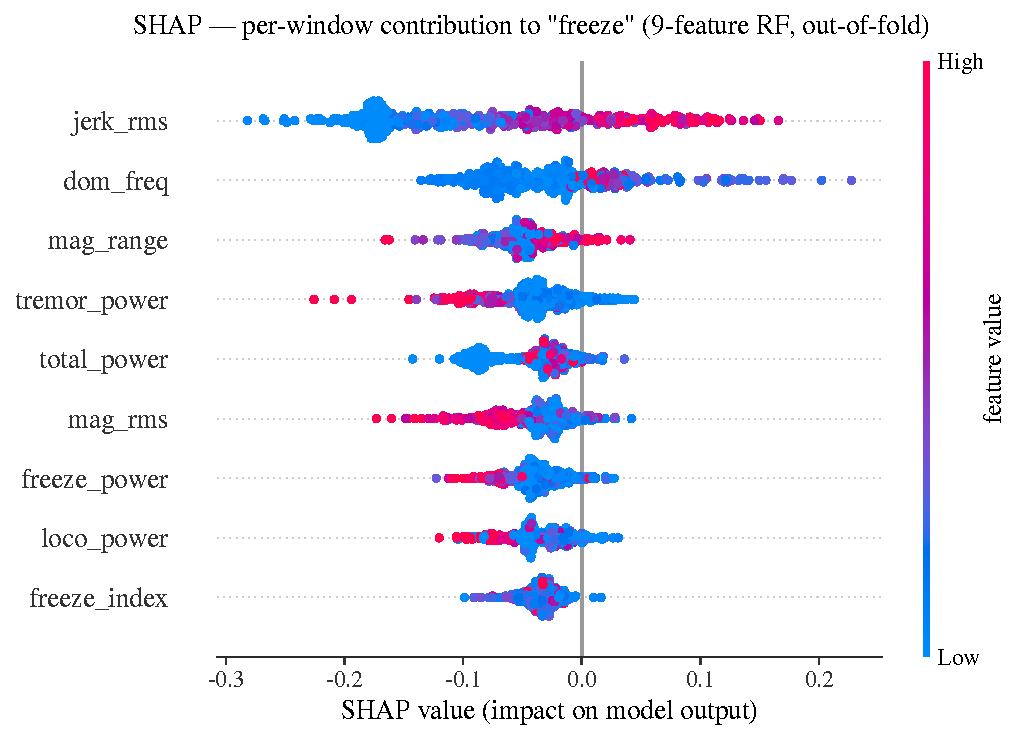
\includegraphics[width=0.74\textwidth]{shap_beeswarm}
  \caption{SHAP beeswarm: each dot is one window; horizontal position is that
  feature's contribution to the freeze score, colour is the feature value (red
  high, blue low). High \feat{jerk\_rms} (red, far right) pushes towards
  ``freeze''; its band is by far the widest.}
  \label{fig:bee}
\end{figure}

\subsection{Shape of the effect, and the Freeze-Index punchline}
Partial dependence (Figure~\ref{fig:pdp}) shows \feat{jerk\_rms} rising
\emph{monotonically} --- more jerk, higher freeze probability --- while
\feat{total\_power} and \feat{freeze\_power} are nearly flat on their own
(consistent with their effect being interaction-driven).

Finally, the teaching punchline: the hand-built \textbf{Freeze Index ranks last}
in \emph{both} PI and SHAP. This is \emph{not} because the $3$--$8$\,Hz band is
irrelevant --- it is because its ingredients (\feat{freeze\_power} and
\feat{loco\_power}) are \emph{already separate features}. A model that can combine
them itself finds the fixed textbook \emph{ratio} redundant. This is a clean,
honest example of feature redundancy --- and of why a learned detector can
outgrow a hand-crafted index, which is the whole reason we use ML here.

\begin{figure}[h]
  \centering
  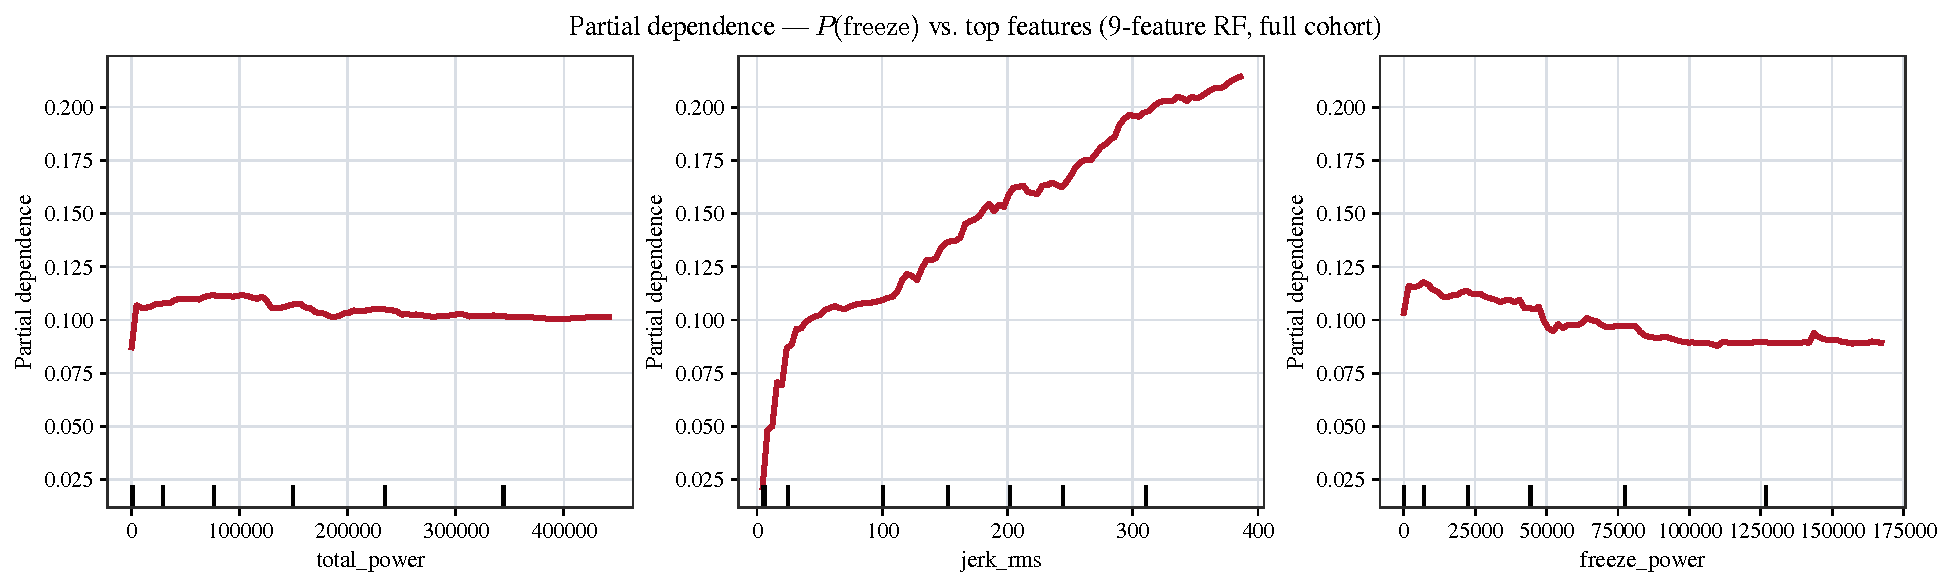
\includegraphics[width=0.95\textwidth]{partial_dependence}
  \caption{Partial dependence of $P(\mathrm{freeze})$ on the top three features.
  \feat{jerk\_rms} (centre) climbs monotonically from $\sim$0.02 to $\sim$0.21;
  \feat{total\_power} and \feat{freeze\_power} are flat marginally --- their
  importance acts through interactions, which a single-feature plot cannot show.}
  \label{fig:pdp}
\end{figure}

\clearpage
% ===========================================================================
\section{How the CNN learns its filters}

The figures so far used the interpretable random forest. This section opens the
\emph{deployed} model --- the 1-D convolutional network FoGNet --- and shows the
four ideas that make it learn: its architecture, the loss it minimises (binary
cross-entropy), the algorithm that minimises it (gradient descent), and what a
real training run actually looks like.

\subsection{Architecture: from a raw window to a freeze probability}
FoGNet takes the raw $3\times256$ accelerometer window and passes it through three
convolutional blocks --- each \emph{learning} its own filters --- then pools and
feeds two small dense layers, ending in two scores that a softmax turns into
$P(\mathrm{freeze})$ (Figure~\ref{fig:cnnarch}). Convolution is the key idea: a
short filter slides along the signal and responds when it meets a local pattern
(a tremor burst, a heel-strike), so the network \emph{discovers} what a freeze
looks like instead of being told. Each max-pool halves the time axis so deeper
filters see longer spans; global average pooling then collapses each of the 64
channels to a single number, which makes the decision robust to \emph{where} in
the window the freeze falls. The whole network is just $18{,}050$ trainable
weights --- small enough to run on the garment's microcontroller.

\begin{figure}[h]
  \centering
  \resizebox{\textwidth}{!}{%
  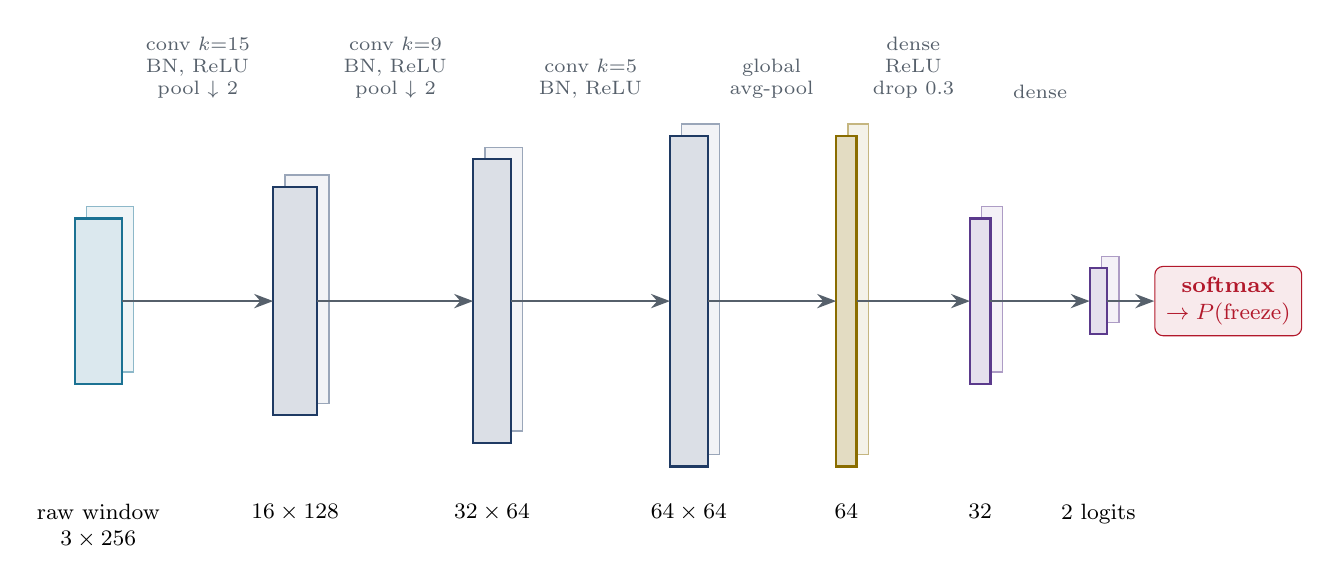
\begin{tikzpicture}[
    inp/.style={draw=cSense, fill=cSense!16, line width=0.8pt},
    inpb/.style={draw=cSense!50, fill=cSense!7, line width=0.5pt},
    vol/.style={draw=navy, fill=navy!16, line width=0.8pt},
    volb/.style={draw=navy!45, fill=navy!6, line width=0.5pt},
    bar/.style={draw=cEval, fill=cEval!24, line width=0.8pt},
    barb/.style={draw=cEval!50, fill=cEval!9, line width=0.5pt},
    den/.style={draw=cInterp, fill=cInterp!16, line width=0.8pt},
    denb/.style={draw=cInterp!50, fill=cInterp!7, line width=0.5pt},
    op/.style={font=\scriptsize, text=mute, align=center, anchor=south,
               text width=1.35cm},
    shp/.style={font=\footnotesize, text=black, align=center, anchor=north},
    fl/.style={-{Stealth[length=2.4mm]}, line width=1pt, mute},
    outbox/.style={draw=freeze, rounded corners=3pt, fill=freeze!9, text=freeze,
                font=\footnotesize\bfseries, align=center, inner sep=4pt},
  ]
    % tensor volumes -- block height grows with channel count
    \cnnvol{0}{0.30}{1.05}{inp}{inpb}
    \cnnvol{2.5}{0.28}{1.45}{vol}{volb}
    \cnnvol{5.0}{0.24}{1.80}{vol}{volb}
    \cnnvol{7.5}{0.24}{2.10}{vol}{volb}
    \cnnvol{9.5}{0.13}{2.10}{bar}{barb}
    \cnnvol{11.2}{0.13}{1.05}{den}{denb}
    \cnnvol{12.7}{0.11}{0.42}{den}{denb}
    \node[outbox] (out) at (14.35,0) {softmax\\$\to P(\mathrm{freeze})$};

    % flow arrows: front-face right edge -> next front-face left edge, at y=0
    \draw[fl] (0.30,0)  -- (2.22,0);
    \draw[fl] (2.78,0)  -- (4.76,0);
    \draw[fl] (5.24,0)  -- (7.26,0);
    \draw[fl] (7.74,0)  -- (9.37,0);
    \draw[fl] (9.63,0)  -- (11.07,0);
    \draw[fl] (11.33,0) -- (12.59,0);
    \draw[fl] (12.81,0) -- (out.west);

    % operation labels (above the arrows)
    \node[op] at (1.26,2.45)  {conv $k{=}15$\\BN, ReLU\\pool $\downarrow2$};
    \node[op] at (3.77,2.45)  {conv $k{=}9$\\BN, ReLU\\pool $\downarrow2$};
    \node[op] at (6.25,2.45)  {conv $k{=}5$\\BN, ReLU};
    \node[op] at (8.55,2.45)  {global\\avg-pool};
    \node[op] at (10.35,2.45) {dense\\ReLU\\drop 0.3};
    \node[op] at (11.96,2.45) {dense};

    % shape labels (below the volumes)
    \node[shp] at (0,-2.45)    {raw window\\$3\times256$};
    \node[shp] at (2.5,-2.45)  {$16\times128$};
    \node[shp] at (5.0,-2.45)  {$32\times64$};
    \node[shp] at (7.5,-2.45)  {$64\times64$};
    \node[shp] at (9.5,-2.45)  {$64$};
    \node[shp] at (11.2,-2.45) {$32$};
    \node[shp] at (12.7,-2.45) {$2$ logits};
  \end{tikzpicture}}
  \caption{\textbf{FoGNet, the deployed detector, end to end.} Block height grows
  with the number of channels (the representation the network builds up); the
  tensor shape (channels\,$\times$\,time) is printed beneath each stage. The three
  convolutional blocks (navy) are the \emph{feature extractor} --- each learns its
  own filters, and the two max-pools halve the time axis ($256\!\to\!128\!\to\!64$).
  Global average pooling (amber) reduces each of the 64 channels to one number; two
  dense layers (purple) form the \emph{classifier head}, ending in two logits that
  the softmax turns into $P(\mathrm{freeze})$. Total: $18{,}050$ learnable weights.}
  \label{fig:cnnarch}
\end{figure}

\subsection{The loss: binary cross-entropy (log-loss)}
Training needs a single number that says \emph{how wrong} the model currently is,
so that ``less wrong'' has a direction to move in. That number is the
\textbf{loss}. For two classes the natural choice is \textbf{binary
cross-entropy} (log-loss): for a window with true label $y\in\{0,1\}$ and
predicted freeze probability $\hat p$,
\[
  \mathcal{L} = -\big[\,y\log\hat p + (1-y)\log(1-\hat p)\,\big].
\]
If the truth is ``freeze'' ($y=1$) this is $-\log\hat p$ --- near zero when the
model confidently says freeze, and \emph{exploding} when it confidently says calm
(Figure~\ref{fig:bce}, left). Being confidently \emph{wrong} is punished far more
than being unsure, which is exactly the incentive a safety detector should have.

\paragraph{Where the probability comes from (the honest detail).}
FoGNet's last layer outputs \emph{two} raw scores (logits), one per class; a
\textbf{softmax} turns them into probabilities that sum to one. With only two
classes the softmax equals the \textbf{sigmoid} of the score difference
$z=z_{\mathrm{freeze}}-z_{\mathrm{calm}}$ (Figure~\ref{fig:bce}, right), and
minimising two-class cross-entropy on the softmax is mathematically identical to
minimising binary cross-entropy on that single freeze probability. We implement
the two-logit form (PyTorch \code{CrossEntropyLoss}) for one practical reason: it
lets us \emph{weight the rare freeze class} directly in the loss --- without that
weighting the model would happily ignore the $9.5\%$ of windows that matter most.
The sigmoid also shows why training can stall: once a score is very large or very
small the curve is flat, its gradient is $\approx 0$, and that window stops
teaching the model anything.

\begin{figure}[h]
  \centering
  \begin{minipage}[t]{0.49\textwidth}
    \centering
    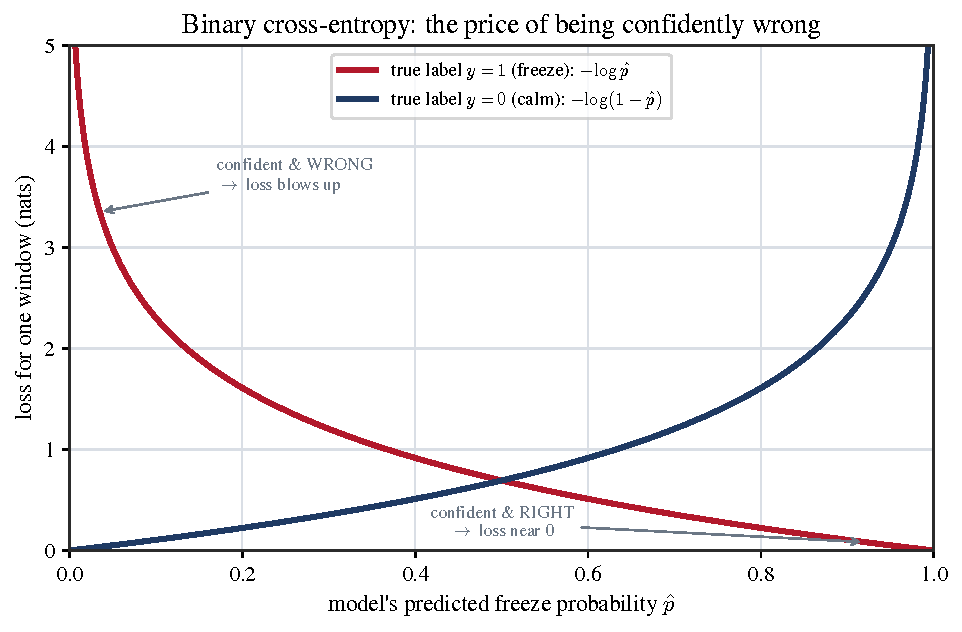
\includegraphics[width=\linewidth]{bce_loss}
    \captionof{figure}{Binary cross-entropy for one window. The loss is small only
    when the model is confident \emph{and} correct; confidently wrong sends it
    sharply upward.}
    \label{fig:bce}
  \end{minipage}\hfill
  \begin{minipage}[t]{0.49\textwidth}
    \centering
    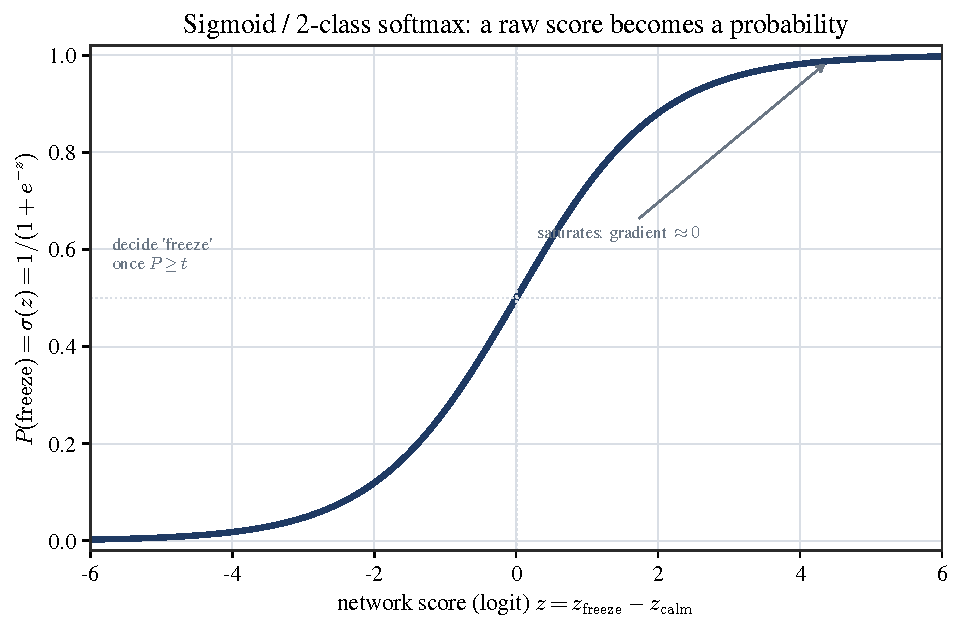
\includegraphics[width=\linewidth]{sigmoid}
    \captionof{figure}{The sigmoid (= 2-class softmax) maps any real score to a
    probability in $(0,1)$. Flat tails mean a vanishing gradient; the threshold
    $t$ is just a vertical cut on this axis.}
    \label{fig:sig}
  \end{minipage}
\end{figure}

\subsection{Learning by gradient descent}
The loss depends on every one of the $18{,}050$ weights at once. \textbf{Training}
means nudging all of them, a little at a time, in the direction that reduces the
loss fastest --- the \emph{negative gradient}, computed for every weight
simultaneously by \textbf{back-propagation}. The size of each nudge is the
\textbf{learning rate}: too small and training crawls; too large and it overshoots
the minimum and zig-zags or diverges (Figure~\ref{fig:gd}). Cadence uses
\textbf{AdamW}, an adaptive optimiser that gives each weight its own effective step
size, with a cosine schedule that shrinks the rate as training proceeds. Real loss
surfaces are not the tidy bowl drawn here --- they live in $18{,}050$ dimensions
and are bumpy --- but the picture (go downhill; mind your step size) is exactly
right.

\begin{figure}[h]
  \centering
  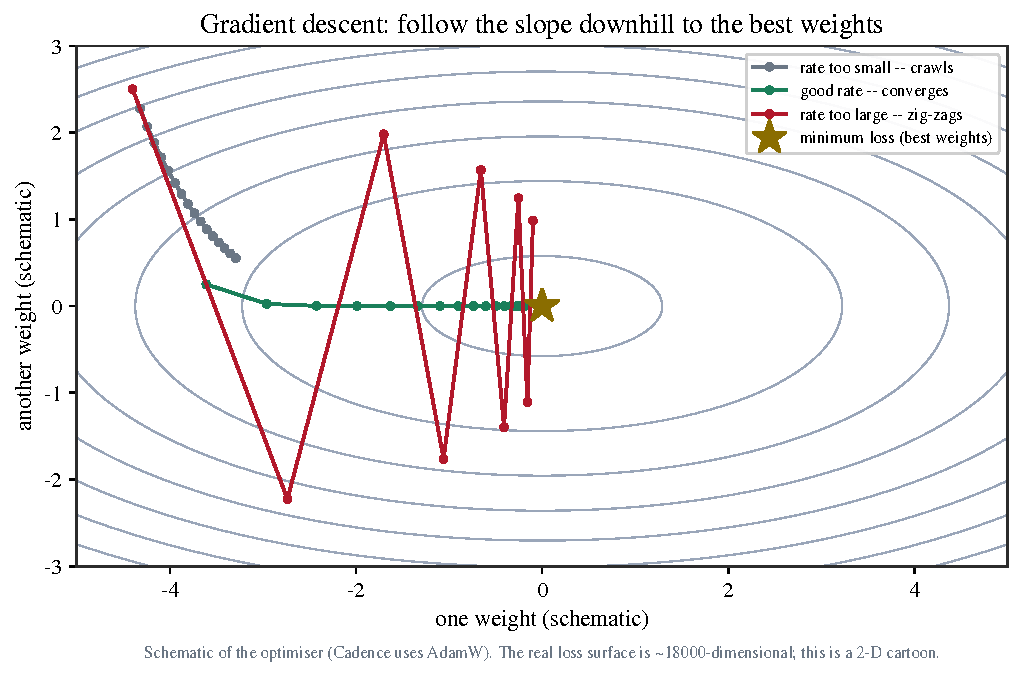
\includegraphics[width=0.66\textwidth]{gradient_descent}
  \caption{Gradient descent on a 2-D toy loss bowl. From the same start, too small
  a rate (grey) barely moves, a good rate (green) slides smoothly to the minimum,
  and too large a rate (red) overshoots and zig-zags. The real optimiser is AdamW
  in $\sim$18\,000 dimensions; this is a schematic of the idea.}
  \label{fig:gd}
\end{figure}

\subsection{Watching it learn --- and knowing when to stop}
Figure~\ref{fig:train} is a \emph{real} FoGNet run on the Daphnet ankle data. The
training loss (red) falls steadily --- the model fits the training windows better
every epoch. But the metric we actually care about, sensitivity on a \emph{held-out}
patient (navy), tells a different story: it climbs, peaks early (epoch~6 here),
then drifts \emph{down} as the network begins to memorise its training subjects
rather than learn the general freeze pattern. This is \textbf{over-fitting}, and
the cure is \textbf{early stopping}: we keep the checkpoint at the validation peak
(gold), not the final epoch. (Our trainer scores checkpoints by
sensitivity\,$+\,0.3\times$specificity, so it leans toward catching freezes.) A
single held-out patient is noisy --- the headline
\textbf{sensitivity $0.71$ / specificity $0.84$} is the average over \emph{all}
patients under leave-one-subject-out, which is the honest estimate for a new wearer.

\begin{figure}[h]
  \centering
  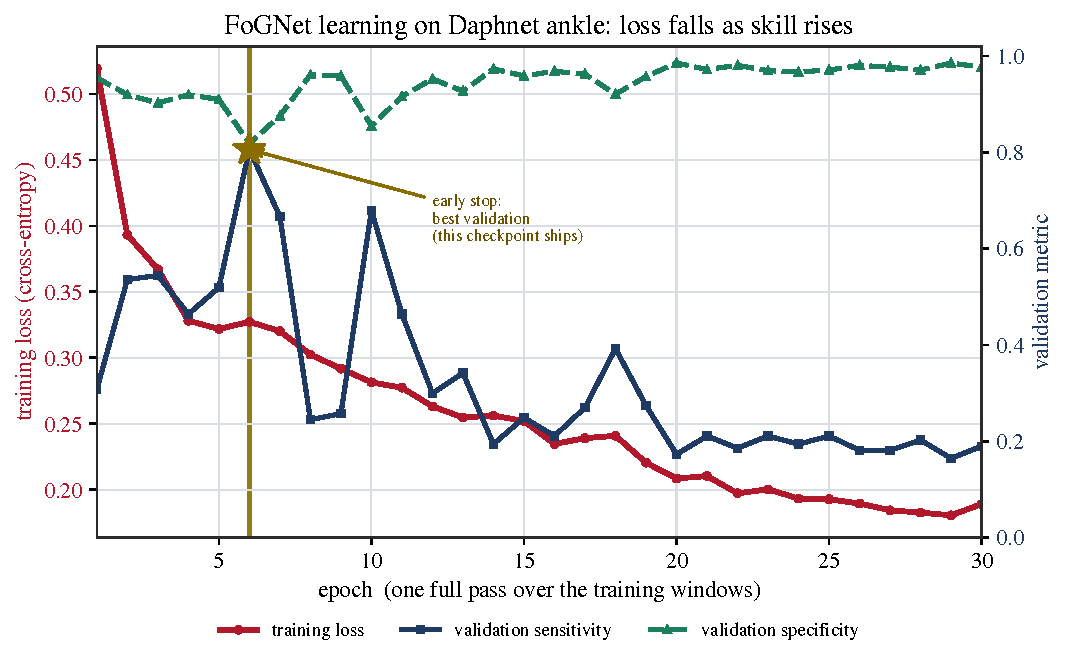
\includegraphics[width=0.86\textwidth]{train_curve}
  \caption{A real FoGNet training run (validation = held-out subject S05). The
  training loss (red, left axis) keeps falling while held-out sensitivity (navy)
  and specificity (green, right axis) plateau and then degrade --- the textbook
  over-fitting signature. The gold marker is the early-stopped checkpoint that is
  actually deployed, not epoch~30. One subject is noisier than the pooled-LOSO
  headline of $0.71/0.84$.}
  \label{fig:train}
\end{figure}

\clearpage
% ===========================================================================
\section{More diagnostic graphs for the detector}

Section~2 introduced the decision threshold; this section shows the full set of
diagnostics behind it. All seven plots use the interpretable 9-feature random
forest evaluated by pooled \textbf{leave-one-subject-out} --- every window is
scored by a model that never saw its own patient (the \emph{out-of-fold}
probabilities). As in \S4 we diagnose the glass box, because its inputs are
physically meaningful; the plots characterise \emph{ranking quality},
\emph{probability honesty}, \emph{per-patient generalisation}, and the
\emph{feature structure} the model has to untangle.

\subsection{Ranking quality, independent of any threshold}
Before fixing a threshold we can ask: does the model \emph{rank} freeze windows
above calm ones? The ROC curve (Figure~\ref{fig:roc}) sweeps every threshold and
plots sensitivity against the false-alarm rate; the area under it (AUC~$=0.82$) is
the probability that a random freeze window scores higher than a random calm one.
Because freezes are rare, the precision--recall curve (Figure~\ref{fig:pr}) is the
more honest view: its baseline is the $9.5\%$ prevalence, and the average precision
(AP~$=0.33$) sits well above that floor. The gold star marks the deployed operating
point ($t\!\approx\!0.10$).

\begin{figure}[h]
  \centering
  \begin{minipage}[t]{0.49\textwidth}
    \centering
    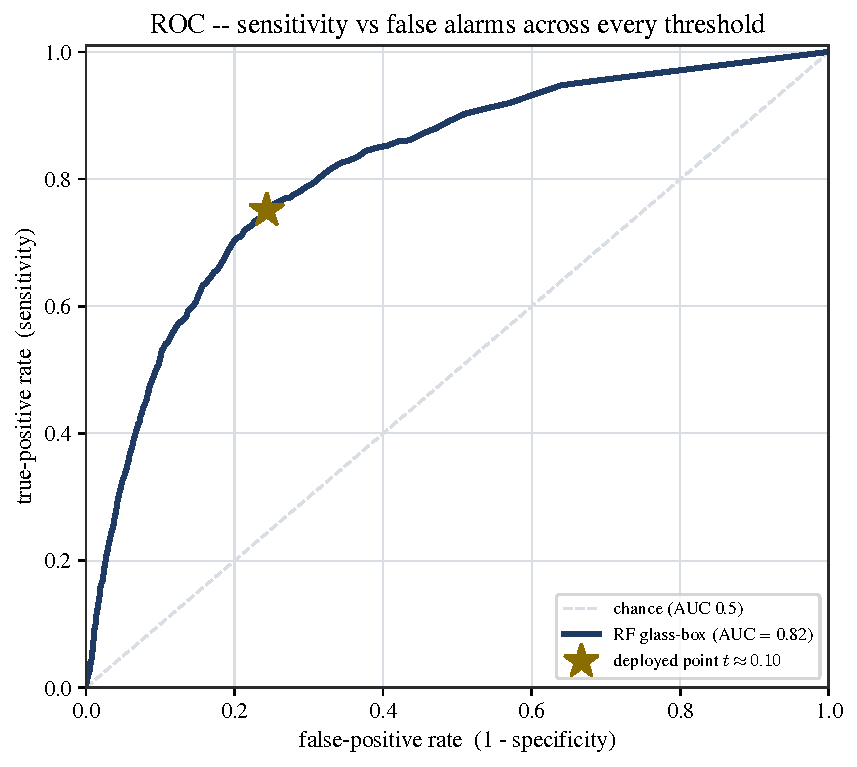
\includegraphics[width=\linewidth]{roc_curve}
    \captionof{figure}{ROC: sensitivity vs false alarms across all thresholds.
    AUC~$=0.82$ --- the chance a random freeze outranks a random calm window. The
    diagonal is coin-flip.}
    \label{fig:roc}
  \end{minipage}\hfill
  \begin{minipage}[t]{0.49\textwidth}
    \centering
    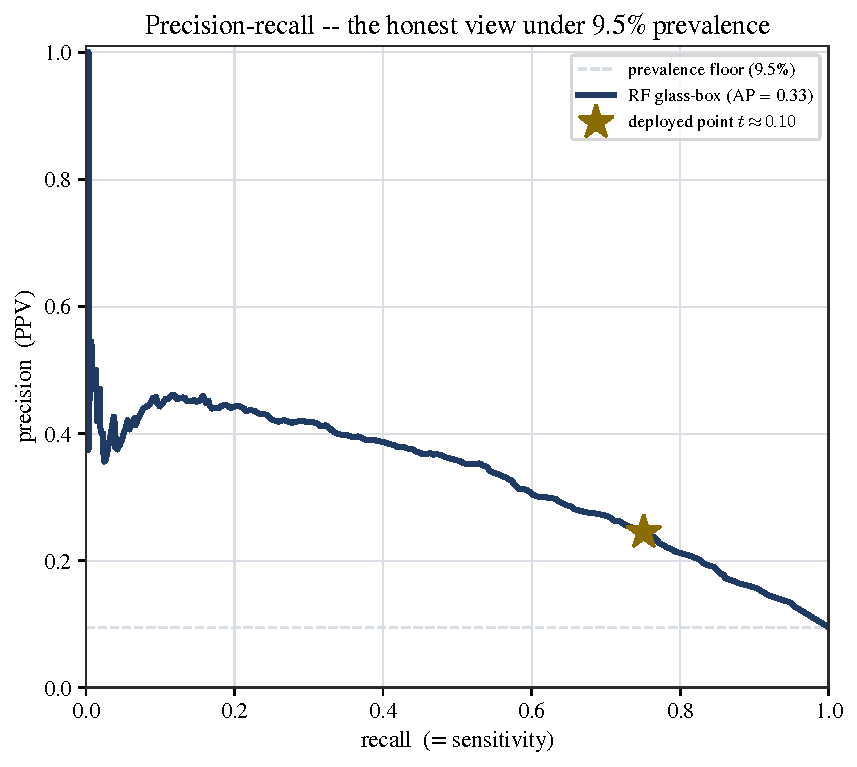
\includegraphics[width=\linewidth]{pr_curve}
    \captionof{figure}{Precision--recall, the honest view under $9.5\%$ prevalence.
    AP~$=0.33$ against a $0.095$ floor; the deployed point trades precision for the
    recall a safety cue needs.}
    \label{fig:pr}
  \end{minipage}
\end{figure}

\subsection{Do the probabilities mean what they say?}
A predicted probability of $0.3$ ought to mean a freeze about $30\%$ of the time.
The reliability diagram (Figure~\ref{fig:cal}) checks this: points on the diagonal
are perfectly calibrated. The forest tracks the diagonal where it has data (the
histogram below shows most windows sit at low probability); the sparse
high-probability bins are noisy, so they are drawn as unconnected dots rather than
joined. Figure~\ref{fig:sh} shows the same scores as two distributions: calm
windows (navy) pile up near zero, freeze windows (red) are pushed right. The
threshold is just a vertical cut --- and because the two piles overlap, no cut
separates them perfectly, which is the real origin of the
sensitivity/specificity trade-off.

\begin{figure}[h]
  \centering
  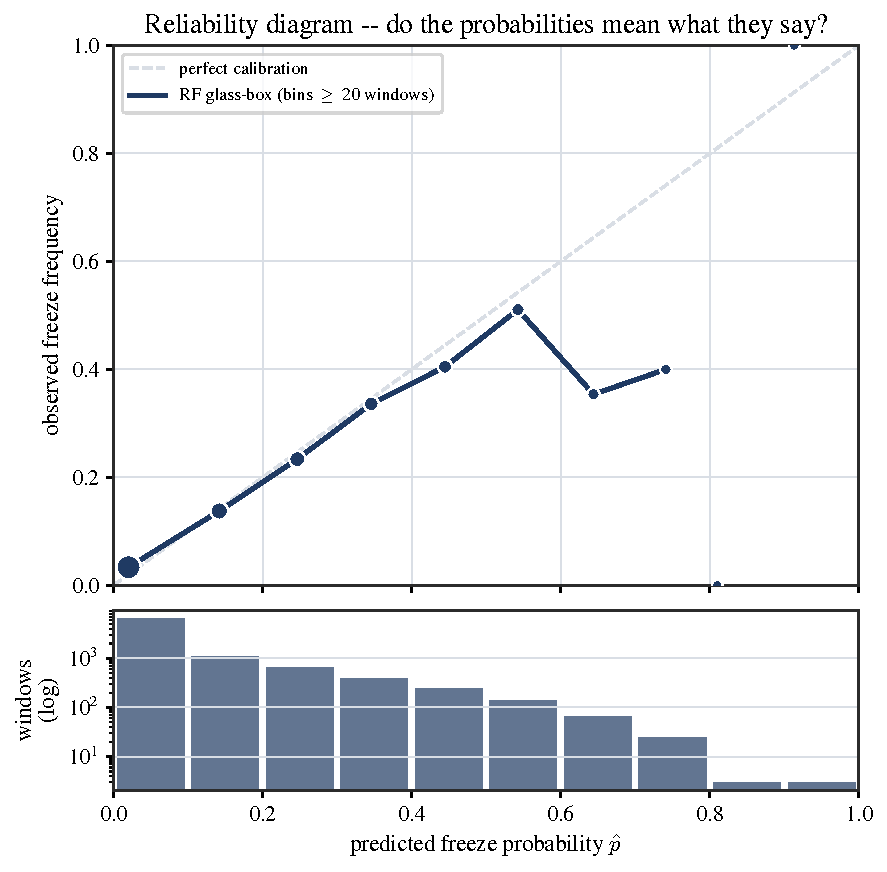
\includegraphics[width=0.56\textwidth]{calibration}
  \caption{Reliability diagram (out-of-fold). Marker size is the number of windows
  in each probability bin; the line is drawn only through bins with $\geq 20$
  windows. The detector is well calibrated where the data live (low probabilities);
  the histogram below confirms how few windows reach high probability.}
  \label{fig:cal}
\end{figure}

\begin{figure}[h]
  \centering
  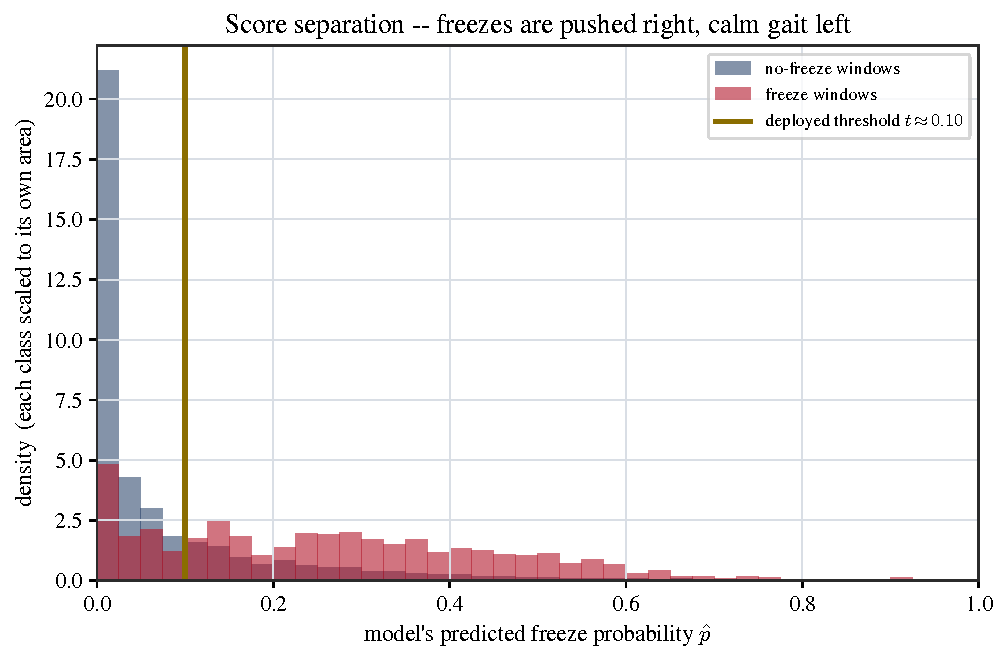
\includegraphics[width=0.70\textwidth]{score_hist}
  \caption{Score separation. The two classes' predicted-probability distributions
  (each scaled to its own area). Freeze windows (red) are pushed right, calm
  windows (navy) cluster near zero; the deployed threshold ($t\!\approx\!0.10$,
  gold) is the cut. The overlap is exactly why a single threshold cannot be both
  perfectly sensitive and perfectly specific.}
  \label{fig:sh}
\end{figure}

\subsection{Does it generalise to a new wearer?}
Pooled numbers can hide a model that works for some patients and fails others.
Figure~\ref{fig:ps} breaks the score down by held-out patient. Most subjects sit
near the pooled lines (sensitivity $0.71$, specificity $0.84$), but the spread is
real --- a reminder that a freeze detector must be validated \emph{per patient},
not just pooled. Two subjects have no labelled freeze windows, so only their
specificity is defined.

\begin{figure}[h]
  \centering
  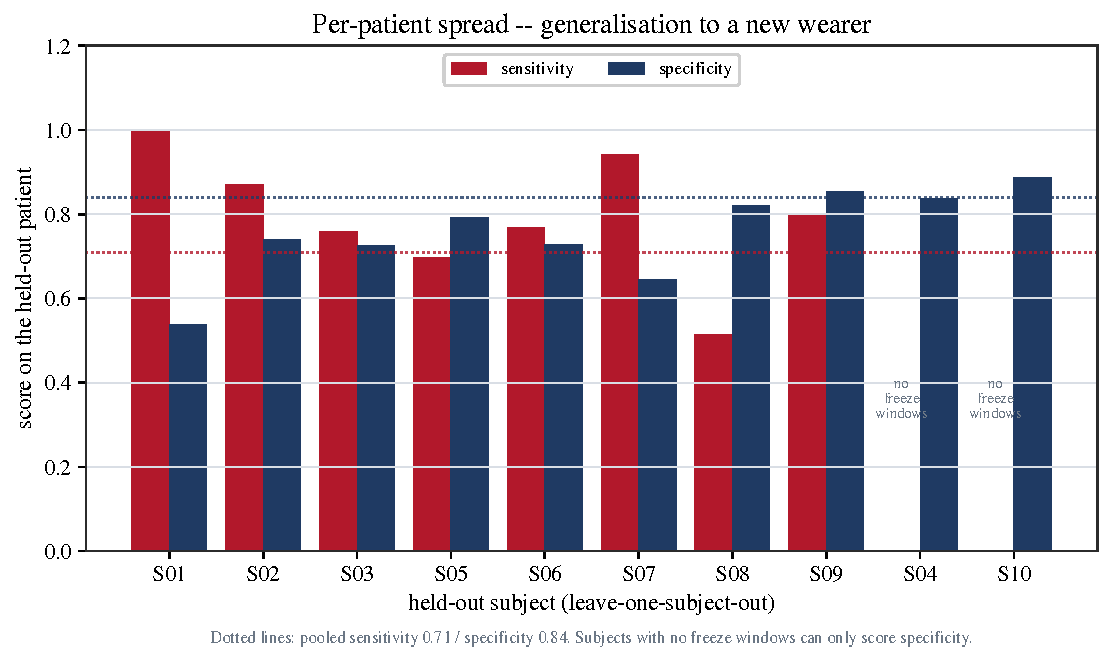
\includegraphics[width=0.90\textwidth]{per_subject}
  \caption{Per-patient sensitivity and specificity under leave-one-subject-out.
  Dotted lines are the pooled headline ($0.71$ / $0.84$). The spread across
  patients is the honest picture of how the garment will behave on an unseen
  wearer.}
  \label{fig:ps}
\end{figure}

\subsection{What the features look like --- and why the Freeze Index is redundant}
Finally, two views of the inputs themselves. The correlation heatmap
(Figure~\ref{fig:fc}) shows heavy redundancy: the four band-power features are
almost perfectly correlated, as are the three magnitude/jerk features. This is
precisely why the model can \emph{reconstruct} the hand-built Freeze Index from its
ingredients and finds the fixed ratio redundant (the punchline of \S4). The box
plots (Figure~\ref{fig:fd}) show \emph{why} the detector works at all: on a freeze
window the jerk is far higher and tighter, total power is higher, and the dominant
frequency shifts --- clean, physical separation between calm gait and freeze.

\begin{figure}[h]
  \centering
  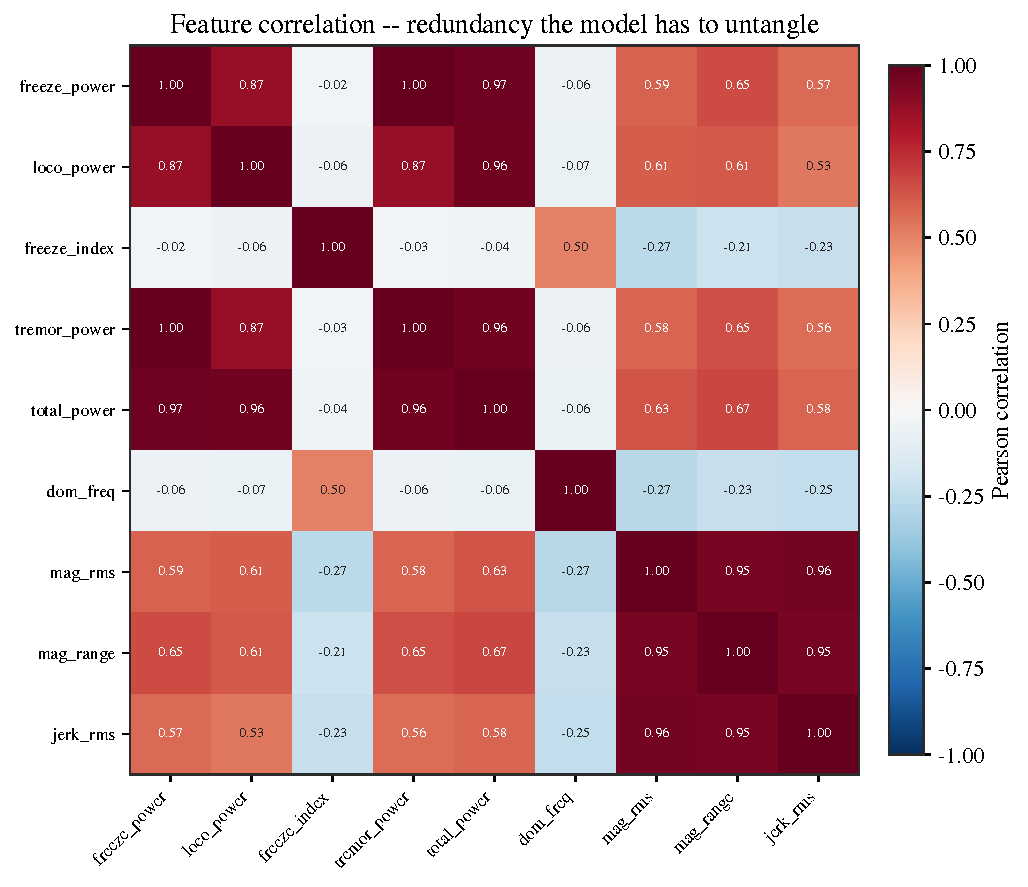
\includegraphics[width=0.58\textwidth]{feature_corr}
  \caption{Pearson correlation between the nine interpretable features. Dark-red
  blocks are near-duplicate features (the band powers; the magnitude/jerk group);
  the Freeze Index correlates only weakly with anything, because its information is
  already carried by its separate ingredients.}
  \label{fig:fc}
\end{figure}

\begin{figure}[h]
  \centering
  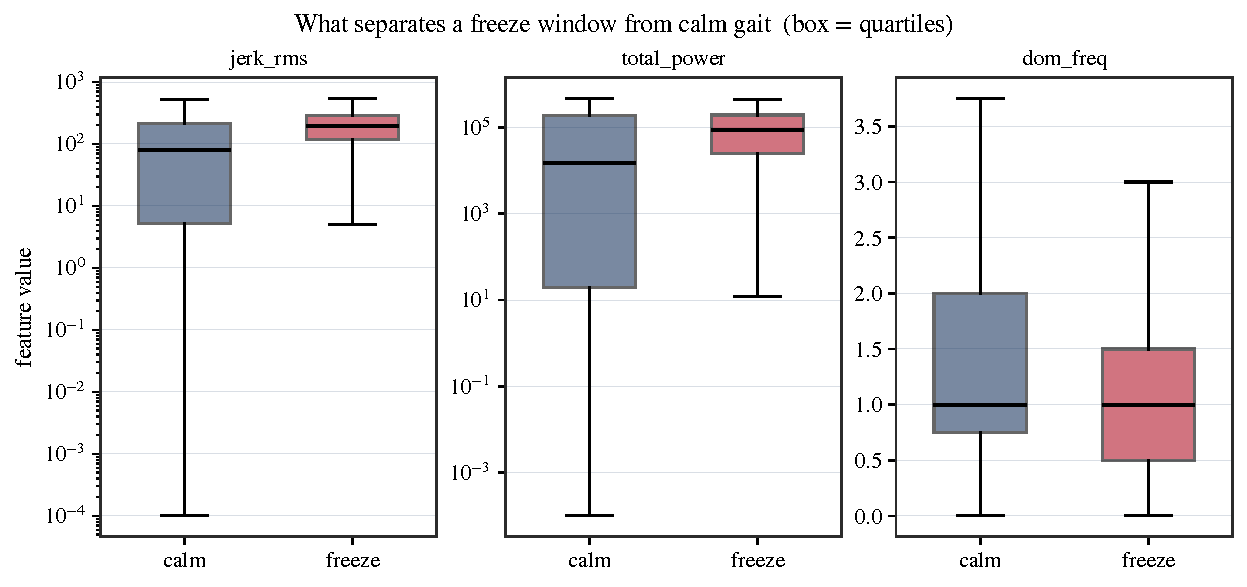
\includegraphics[width=0.92\textwidth]{feature_dist}
  \caption{Class-conditional box plots (quartiles, whiskers to the
  $5$th/$95$th percentile) for three telling features. Jerk and total power are log
  scaled. The freeze boxes (red) are clearly shifted from the calm boxes (navy) ---
  this separation is what every model in this document is exploiting.}
  \label{fig:fd}
\end{figure}

\vspace{4pt}
\begin{center}
\fcolorbox{navy}{navy!6}{%
\begin{minipage}{0.95\textwidth}
\textbf{\color{navy}What we deploy, and what we headline.}\;
The \emph{deployed} detector is the 1-D CNN; the random forest is the glass box
behind these interpretation plots. We headline \textbf{sensitivity $0.71$ /
specificity $0.84$} (CNN, leave-one-subject-out), with the decision threshold
chosen by \emph{nested} LOSO so the figures hold for a new patient. The model's
strongest learned cue is ankle \emph{jerk} --- and it has, sensibly, learned to
outgrow the textbook Freeze Index.
\end{minipage}}
\end{center}

\vfill
{\color{mute}\footnotesize
\noindent\textbf{Reproducibility.} Every number and figure is generated from the
public Daphnet FoG benchmark (ankle sensor) by:
\begin{itemize}[leftmargin=1.6em,itemsep=1pt]
  \item \code{colab/fog\_allinone.py} --- CNN training \& leave-one-subject-out predictions;
  \item \code{pi/make\_accuracy\_figs.py} --- confusion matrix, metric panel, accuracy caveat, SHAP, permutation importance, partial dependence;
  \item \code{pi/make\_cnn\_figs.py} --- the real FoGNet training curve plus the loss/sigmoid/gradient-descent schematics and the ROC, precision--recall, calibration, score-separation, per-subject and feature diagnostics;
  \item \code{pi/make\_decision\_figs.py} --- decision contour, parameter grid, operating point;
  \item \code{colab/pick\_threshold.py} --- nested-LOSO threshold selection.
\end{itemize}}

\end{document}
